\documentclass[twoside]{book}

% Packages required by doxygen
\usepackage{fixltx2e}
\usepackage{calc}
\usepackage{doxygen}
\usepackage[export]{adjustbox} % also loads graphicx
\usepackage{graphicx}
\usepackage[utf8]{inputenc}
\usepackage{makeidx}
\usepackage{multicol}
\usepackage{multirow}
\PassOptionsToPackage{warn}{textcomp}
\usepackage{textcomp}
\usepackage[nointegrals]{wasysym}
\usepackage[table]{xcolor}

% Font selection
\usepackage[T1]{fontenc}
\usepackage[scaled=.90]{helvet}
\usepackage{courier}
\usepackage{amssymb}
\usepackage{sectsty}
\renewcommand{\familydefault}{\sfdefault}
\allsectionsfont{%
  \fontseries{bc}\selectfont%
  \color{darkgray}%
}
\renewcommand{\DoxyLabelFont}{%
  \fontseries{bc}\selectfont%
  \color{darkgray}%
}
\newcommand{\+}{\discretionary{\mbox{\scriptsize$\hookleftarrow$}}{}{}}

% Page & text layout
\usepackage{geometry}
\geometry{%
  letterpaper,%
  top=2.5cm,%
  bottom=2.5cm,%
  left=2.5cm,%
  right=2.5cm%
}
\tolerance=750
\hfuzz=15pt
\hbadness=750
\setlength{\emergencystretch}{15pt}
\setlength{\parindent}{0cm}
\setlength{\parskip}{3ex plus 2ex minus 2ex}
\makeatletter
\renewcommand{\paragraph}{%
  \@startsection{paragraph}{4}{0ex}{-1.0ex}{1.0ex}{%
    \normalfont\normalsize\bfseries\SS@parafont%
  }%
}
\renewcommand{\subparagraph}{%
  \@startsection{subparagraph}{5}{0ex}{-1.0ex}{1.0ex}{%
    \normalfont\normalsize\bfseries\SS@subparafont%
  }%
}
\makeatother

% Headers & footers
\usepackage{fancyhdr}
\pagestyle{fancyplain}
\fancyhead[LE]{\fancyplain{}{\bfseries\thepage}}
\fancyhead[CE]{\fancyplain{}{}}
\fancyhead[RE]{\fancyplain{}{\bfseries\leftmark}}
\fancyhead[LO]{\fancyplain{}{\bfseries\rightmark}}
\fancyhead[CO]{\fancyplain{}{}}
\fancyhead[RO]{\fancyplain{}{\bfseries\thepage}}
\fancyfoot[LE]{\fancyplain{}{}}
\fancyfoot[CE]{\fancyplain{}{}}
\fancyfoot[RE]{\fancyplain{}{\bfseries\scriptsize Generated by Doxygen }}
\fancyfoot[LO]{\fancyplain{}{\bfseries\scriptsize Generated by Doxygen }}
\fancyfoot[CO]{\fancyplain{}{}}
\fancyfoot[RO]{\fancyplain{}{}}
\renewcommand{\footrulewidth}{0.4pt}
\renewcommand{\chaptermark}[1]{%
  \markboth{#1}{}%
}
\renewcommand{\sectionmark}[1]{%
  \markright{\thesection\ #1}%
}

% Indices & bibliography
\usepackage{natbib}
\usepackage[titles]{tocloft}
\setcounter{tocdepth}{3}
\setcounter{secnumdepth}{5}
\makeindex

% Hyperlinks (required, but should be loaded last)
\usepackage{ifpdf}
\ifpdf
  \usepackage[pdftex,pagebackref=true]{hyperref}
\else
  \usepackage[ps2pdf,pagebackref=true]{hyperref}
\fi
\hypersetup{%
  colorlinks=true,%
  linkcolor=blue,%
  citecolor=blue,%
  unicode%
}

% Custom commands
\newcommand{\clearemptydoublepage}{%
  \newpage{\pagestyle{empty}\cleardoublepage}%
}

\usepackage{caption}
\captionsetup{labelsep=space,justification=centering,font={bf},singlelinecheck=off,skip=4pt,position=top}

%===== C O N T E N T S =====

\begin{document}

% Titlepage & ToC
\hypersetup{pageanchor=false,
             bookmarksnumbered=true,
             pdfencoding=unicode
            }
\pagenumbering{alph}
\begin{titlepage}
\vspace*{7cm}
\begin{center}%
{\Large M\+E-\/507 Term Project\+: Ball Fetching Car \\[1ex]\large V0.\+9 }\\
\vspace*{1cm}
{\large Generated by Doxygen 1.8.14}\\
\end{center}
\end{titlepage}
\clearemptydoublepage
\pagenumbering{roman}
\tableofcontents
\clearemptydoublepage
\pagenumbering{arabic}
\hypersetup{pageanchor=true}

%--- Begin generated contents ---
\chapter{Hierarchical Index}
\section{Class Hierarchy}
This inheritance list is sorted roughly, but not completely, alphabetically\+:\begin{DoxyCompactList}
\item Task\+Base\begin{DoxyCompactList}
\item \contentsline{section}{task\+\_\+car\+\_\+control}{\pageref{classtask__car__control}}{}
\item \contentsline{section}{task\+\_\+motor}{\pageref{classtask__motor}}{}
\item \contentsline{section}{task\+\_\+radio}{\pageref{classtask__radio}}{}
\item \contentsline{section}{task\+\_\+steering}{\pageref{classtask__steering}}{}
\item \contentsline{section}{task\+\_\+user}{\pageref{classtask__user}}{}
\item \contentsline{section}{task\+\_\+\+U\+S\+R1}{\pageref{classtask__USR1}}{}
\end{DoxyCompactList}
\end{DoxyCompactList}

\chapter{Class Index}
\section{Class List}
Here are the classes, structs, unions and interfaces with brief descriptions\+:\begin{DoxyCompactList}
\item\contentsline{section}{\mbox{\hyperlink{classtask__car__control}{task\+\_\+car\+\_\+control}} \\*This task is used to control movement of the car }{\pageref{classtask__car__control}}{}
\item\contentsline{section}{\mbox{\hyperlink{classtask__motor}{task\+\_\+motor}} \\*This task is used to control the velocity of the motor }{\pageref{classtask__motor}}{}
\item\contentsline{section}{\mbox{\hyperlink{classtask__radio}{task\+\_\+radio}} \\*This task is used to control the RF transciever }{\pageref{classtask__radio}}{}
\item\contentsline{section}{\mbox{\hyperlink{classtask__steering}{task\+\_\+steering}} \\*This task is used to control the position of the servo }{\pageref{classtask__steering}}{}
\item\contentsline{section}{\mbox{\hyperlink{classtask__user}{task\+\_\+user}} \\*This task is used to create a user interface to communicate with }{\pageref{classtask__user}}{}
\item\contentsline{section}{\mbox{\hyperlink{classtask__USR1}{task\+\_\+\+U\+S\+R1}} }{\pageref{classtask__USR1}}{}
\end{DoxyCompactList}

\chapter{File Index}
\section{File List}
Here is a list of all documented files with brief descriptions\+:\begin{DoxyCompactList}
\item\contentsline{section}{\mbox{\hyperlink{main_8cpp}{main.\+cpp}} }{\pageref{main_8cpp}}{}
\item\contentsline{section}{{\bfseries nrf\+\_\+names.\+h} }{\pageref{nrf__names_8h}}{}
\item\contentsline{section}{\mbox{\hyperlink{shares_8h}{shares.\+h}} }{\pageref{shares_8h}}{}
\item\contentsline{section}{\mbox{\hyperlink{task__car__control_8cpp}{task\+\_\+car\+\_\+control.\+cpp}} }{\pageref{task__car__control_8cpp}}{}
\item\contentsline{section}{\mbox{\hyperlink{task__car__control_8h}{task\+\_\+car\+\_\+control.\+h}} }{\pageref{task__car__control_8h}}{}
\item\contentsline{section}{\mbox{\hyperlink{task__motor_8cpp}{task\+\_\+motor.\+cpp}} }{\pageref{task__motor_8cpp}}{}
\item\contentsline{section}{\mbox{\hyperlink{task__motor_8h}{task\+\_\+motor.\+h}} }{\pageref{task__motor_8h}}{}
\item\contentsline{section}{\mbox{\hyperlink{task__radio_8cpp}{task\+\_\+radio.\+cpp}} }{\pageref{task__radio_8cpp}}{}
\item\contentsline{section}{\mbox{\hyperlink{task__radio_8h}{task\+\_\+radio.\+h}} }{\pageref{task__radio_8h}}{}
\item\contentsline{section}{\mbox{\hyperlink{task__steering_8cpp}{task\+\_\+steering.\+cpp}} }{\pageref{task__steering_8cpp}}{}
\item\contentsline{section}{\mbox{\hyperlink{task__steering_8h}{task\+\_\+steering.\+h}} }{\pageref{task__steering_8h}}{}
\item\contentsline{section}{\mbox{\hyperlink{task__user_8cpp}{task\+\_\+user.\+cpp}} }{\pageref{task__user_8cpp}}{}
\item\contentsline{section}{\mbox{\hyperlink{task__user_8h}{task\+\_\+user.\+h}} }{\pageref{task__user_8h}}{}
\item\contentsline{section}{\mbox{\hyperlink{task__USR1_8cpp}{task\+\_\+\+U\+S\+R1.\+cpp}} }{\pageref{task__USR1_8cpp}}{}
\item\contentsline{section}{\mbox{\hyperlink{task__USR1_8h}{task\+\_\+\+U\+S\+R1.\+h}} }{\pageref{task__USR1_8h}}{}
\end{DoxyCompactList}

\chapter{Class Documentation}
\hypertarget{classtask__car__control}{}\section{task\+\_\+car\+\_\+control Class Reference}
\label{classtask__car__control}\index{task\+\_\+car\+\_\+control@{task\+\_\+car\+\_\+control}}


This task is used to control movement of the car.  




{\ttfamily \#include $<$task\+\_\+car\+\_\+control.\+h$>$}

Inheritance diagram for task\+\_\+car\+\_\+control\+:\begin{figure}[H]
\begin{center}
\leavevmode
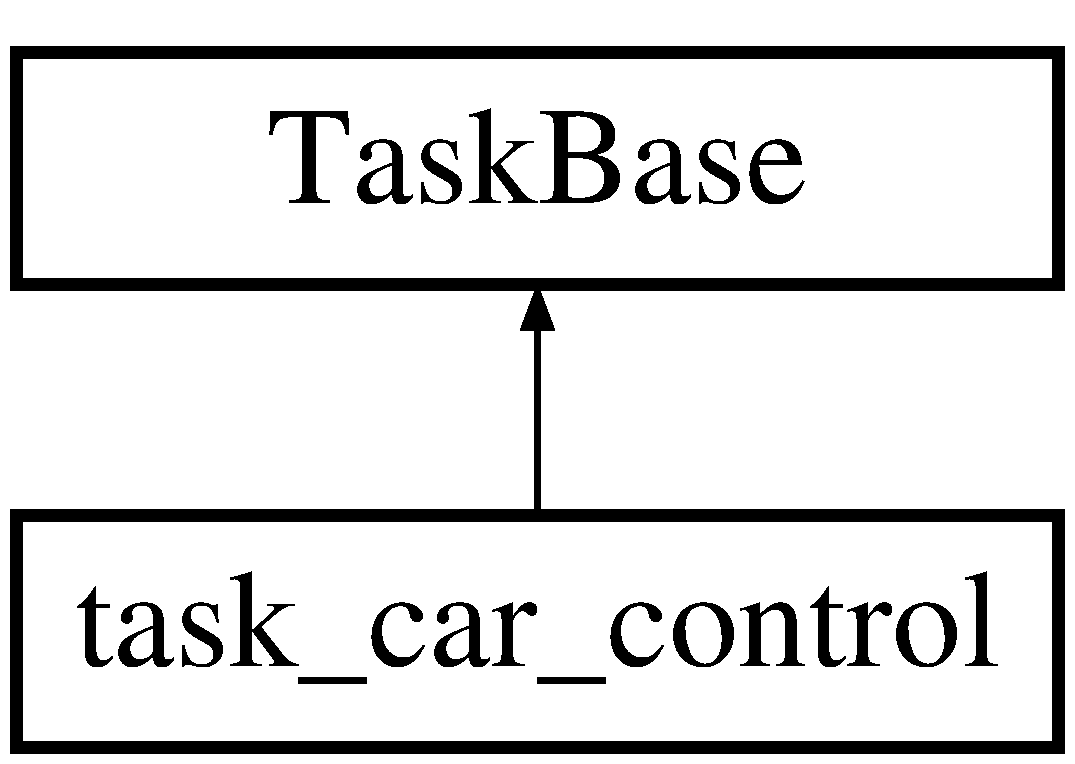
\includegraphics[height=2.000000cm]{classtask__car__control}
\end{center}
\end{figure}
\subsection*{Public Member Functions}
\begin{DoxyCompactItemize}
\item 
\mbox{\hyperlink{classtask__car__control_ae42d6364ed49d5d59a5d3dbebc8a7f38}{task\+\_\+car\+\_\+control}} (const char $\ast$, unsigned port\+B\+A\+S\+E\+\_\+\+T\+Y\+PE, size\+\_\+t, emstream $\ast$)
\item 
void \mbox{\hyperlink{classtask__car__control_a797dbdeb270271b48c468442d3ab91bd}{run}} (void)
\begin{DoxyCompactList}\small\item\em This method is called to actuate the motor and servo. \end{DoxyCompactList}\end{DoxyCompactItemize}


\subsection{Detailed Description}
This task is used to control movement of the car. 

This task inherits the Task\+Base class, and is used to run as a finite state machine. It controls the actions of the motor and servo using shared variables. 

Definition at line 56 of file task\+\_\+car\+\_\+control.\+h.



\subsection{Constructor \& Destructor Documentation}
\mbox{\Hypertarget{classtask__car__control_ae42d6364ed49d5d59a5d3dbebc8a7f38}\label{classtask__car__control_ae42d6364ed49d5d59a5d3dbebc8a7f38}} 
\index{task\+\_\+car\+\_\+control@{task\+\_\+car\+\_\+control}!task\+\_\+car\+\_\+control@{task\+\_\+car\+\_\+control}}
\index{task\+\_\+car\+\_\+control@{task\+\_\+car\+\_\+control}!task\+\_\+car\+\_\+control@{task\+\_\+car\+\_\+control}}
\subsubsection{\texorpdfstring{task\+\_\+car\+\_\+control()}{task\_car\_control()}}
{\footnotesize\ttfamily task\+\_\+car\+\_\+control\+::task\+\_\+car\+\_\+control (\begin{DoxyParamCaption}\item[{const char $\ast$}]{a\+\_\+name,  }\item[{unsigned port\+B\+A\+S\+E\+\_\+\+T\+Y\+PE}]{a\+\_\+priority,  }\item[{size\+\_\+t}]{a\+\_\+stack\+\_\+size,  }\item[{emstream $\ast$}]{p\+\_\+ser\+\_\+dev }\end{DoxyParamCaption})}

This constructor creates a task to control the actions of the car. It is used to control the motor setpoint and the servo setpoint. 
\begin{DoxyParams}{Parameters}
{\em a\+\_\+name} & A character string which will be the name of this task \\
\hline
{\em a\+\_\+priority} & The priority at which this task will initially run (default\+: 0) \\
\hline
{\em a\+\_\+stack\+\_\+size} & The size of this task\textquotesingle{}s stack in bytes (default\+: config\+M\+I\+N\+I\+M\+A\+L\+\_\+\+S\+T\+A\+C\+K\+\_\+\+S\+I\+ZE) \\
\hline
{\em p\+\_\+ser\+\_\+dev} & A pointer to the serial port which writes debugging info. \\
\hline
\end{DoxyParams}


Definition at line 32 of file task\+\_\+car\+\_\+control.\+cpp.



\subsection{Member Function Documentation}
\mbox{\Hypertarget{classtask__car__control_a797dbdeb270271b48c468442d3ab91bd}\label{classtask__car__control_a797dbdeb270271b48c468442d3ab91bd}} 
\index{task\+\_\+car\+\_\+control@{task\+\_\+car\+\_\+control}!run@{run}}
\index{run@{run}!task\+\_\+car\+\_\+control@{task\+\_\+car\+\_\+control}}
\subsubsection{\texorpdfstring{run()}{run()}}
{\footnotesize\ttfamily void task\+\_\+car\+\_\+control\+::run (\begin{DoxyParamCaption}\item[{void}]{ }\end{DoxyParamCaption})}



This method is called to actuate the motor and servo. 

This method is called by the R\+T\+OS once to run the task loop for ever and ever.

This function works within the Free\+R\+T\+OS framework. Once it is called, it loops through a switch for as long as the main program is running in a finite state machine. This task uses the shared p\+\_\+motor\+\_\+vel and p\+\_\+servo\+\_\+pos variables calculate to get the car to move as desired. 

Definition at line 52 of file task\+\_\+car\+\_\+control.\+cpp.



References p\+\_\+drive\+\_\+state, p\+\_\+motor\+\_\+vel, p\+\_\+servo\+\_\+pos, and width\+\_\+1.



The documentation for this class was generated from the following files\+:\begin{DoxyCompactItemize}
\item 
\mbox{\hyperlink{task__car__control_8h}{task\+\_\+car\+\_\+control.\+h}}\item 
\mbox{\hyperlink{task__car__control_8cpp}{task\+\_\+car\+\_\+control.\+cpp}}\end{DoxyCompactItemize}

\hypertarget{classtask__motor}{}\section{task\+\_\+motor Class Reference}
\label{classtask__motor}\index{task\+\_\+motor@{task\+\_\+motor}}


This task is used to control the velocity of the motor.  




{\ttfamily \#include $<$task\+\_\+motor.\+h$>$}

Inheritance diagram for task\+\_\+motor\+:\begin{figure}[H]
\begin{center}
\leavevmode
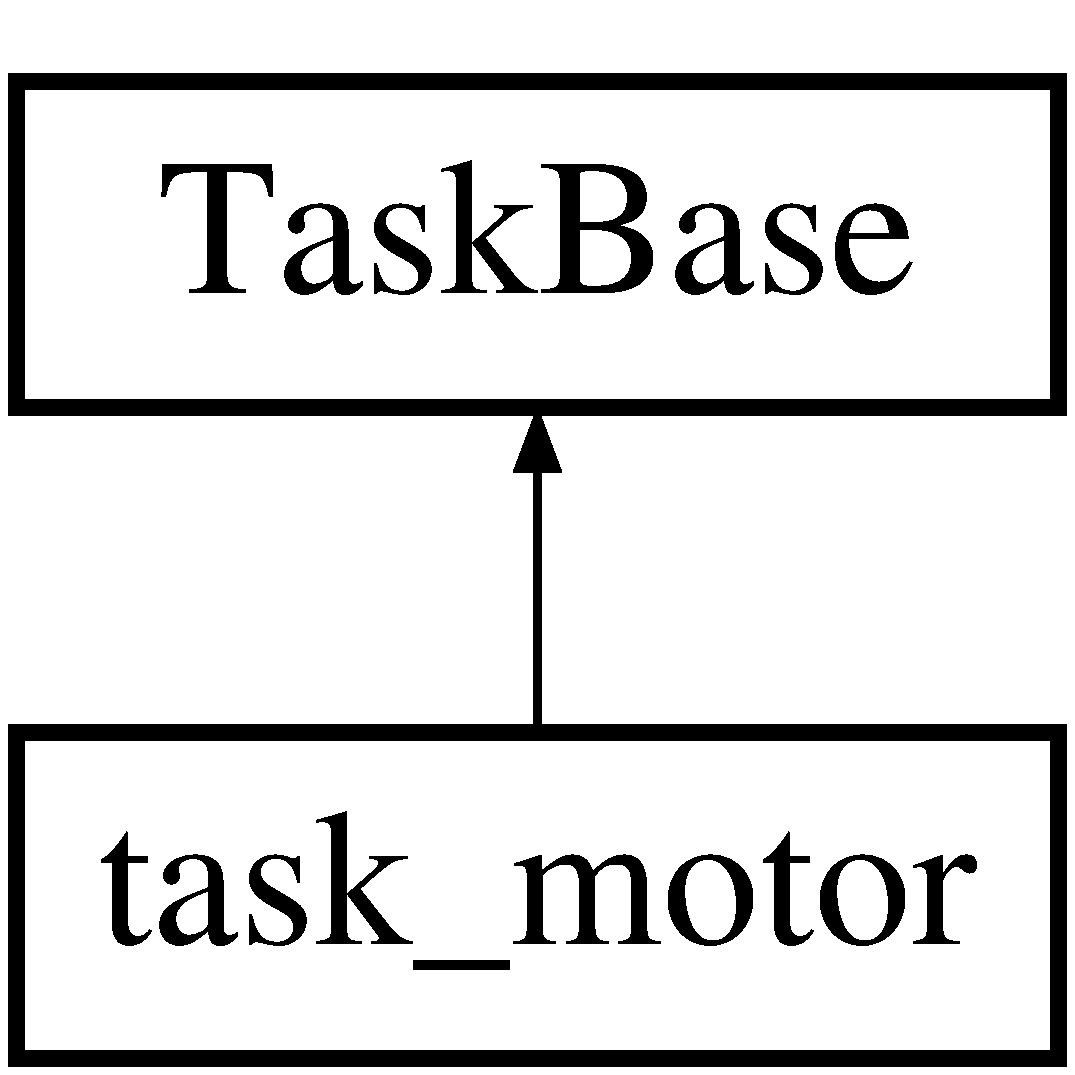
\includegraphics[height=2.000000cm]{classtask__motor}
\end{center}
\end{figure}
\subsection*{Public Member Functions}
\begin{DoxyCompactItemize}
\item 
\mbox{\hyperlink{classtask__motor_a6ed0a0b463e698d636b28bcdd518a027}{task\+\_\+motor}} (const char $\ast$, unsigned port\+B\+A\+S\+E\+\_\+\+T\+Y\+PE, size\+\_\+t, emstream $\ast$)
\item 
void \mbox{\hyperlink{classtask__motor_a895a075ec470c9d5a07b8959de06aacd}{run}} (void)
\begin{DoxyCompactList}\small\item\em This method is called to run the motor control loop. \end{DoxyCompactList}\end{DoxyCompactItemize}
\subsection*{Protected Member Functions}
\begin{DoxyCompactItemize}
\item 
uint8\+\_\+t \mbox{\hyperlink{classtask__motor_a6022366bdc25c0a1c16b96bbc02bcffa}{calc\+\_\+pwm}} (int8\+\_\+t)
\begin{DoxyCompactList}\small\item\em This method calculates the P\+WM length to be sent to the timer. \end{DoxyCompactList}\end{DoxyCompactItemize}
\subsection*{Protected Attributes}
\begin{DoxyCompactItemize}
\item 
\mbox{\Hypertarget{classtask__motor_a7ccbea1fe01e35b055688cca8b5be8f0}\label{classtask__motor_a7ccbea1fe01e35b055688cca8b5be8f0}} 
int8\+\_\+t \mbox{\hyperlink{classtask__motor_a7ccbea1fe01e35b055688cca8b5be8f0}{offset}}
\begin{DoxyCompactList}\small\item\em This value is used to set the offset from zero so that the motor does not move when set to 0 velocity. \end{DoxyCompactList}\end{DoxyCompactItemize}


\subsection{Detailed Description}
This task is used to control the velocity of the motor. 

This task inherits the Task\+Base class, and is used to run as a finite state machine. It controls the actions of the motor using a timer for P\+WM. 

Definition at line 55 of file task\+\_\+motor.\+h.



\subsection{Constructor \& Destructor Documentation}
\mbox{\Hypertarget{classtask__motor_a6ed0a0b463e698d636b28bcdd518a027}\label{classtask__motor_a6ed0a0b463e698d636b28bcdd518a027}} 
\index{task\+\_\+motor@{task\+\_\+motor}!task\+\_\+motor@{task\+\_\+motor}}
\index{task\+\_\+motor@{task\+\_\+motor}!task\+\_\+motor@{task\+\_\+motor}}
\subsubsection{\texorpdfstring{task\+\_\+motor()}{task\_motor()}}
{\footnotesize\ttfamily task\+\_\+motor\+::task\+\_\+motor (\begin{DoxyParamCaption}\item[{const char $\ast$}]{a\+\_\+name,  }\item[{unsigned port\+B\+A\+S\+E\+\_\+\+T\+Y\+PE}]{a\+\_\+priority,  }\item[{size\+\_\+t}]{a\+\_\+stack\+\_\+size,  }\item[{emstream $\ast$}]{p\+\_\+ser\+\_\+dev }\end{DoxyParamCaption})}

This constructor creates a task to control the motor velocity. It is used to control the forward movement of the car. 
\begin{DoxyParams}{Parameters}
{\em a\+\_\+name} & A character string which will be the name of this task \\
\hline
{\em a\+\_\+priority} & The priority at which this task will initially run (default\+: 0) \\
\hline
{\em a\+\_\+stack\+\_\+size} & The size of this task\textquotesingle{}s stack in bytes (default\+: config\+M\+I\+N\+I\+M\+A\+L\+\_\+\+S\+T\+A\+C\+K\+\_\+\+S\+I\+ZE) \\
\hline
{\em p\+\_\+ser\+\_\+dev} & A pointer to the serial port which writes debugging info. \\
\hline
\end{DoxyParams}


Definition at line 45 of file task\+\_\+motor.\+cpp.



\subsection{Member Function Documentation}
\mbox{\Hypertarget{classtask__motor_a6022366bdc25c0a1c16b96bbc02bcffa}\label{classtask__motor_a6022366bdc25c0a1c16b96bbc02bcffa}} 
\index{task\+\_\+motor@{task\+\_\+motor}!calc\+\_\+pwm@{calc\+\_\+pwm}}
\index{calc\+\_\+pwm@{calc\+\_\+pwm}!task\+\_\+motor@{task\+\_\+motor}}
\subsubsection{\texorpdfstring{calc\+\_\+pwm()}{calc\_pwm()}}
{\footnotesize\ttfamily uint8\+\_\+t task\+\_\+motor\+::calc\+\_\+pwm (\begin{DoxyParamCaption}\item[{int8\+\_\+t}]{pwm }\end{DoxyParamCaption})\hspace{0.3cm}{\ttfamily [protected]}}



This method calculates the P\+WM length to be sent to the timer. 

This method takes a single input of the desired motor velocity. From this value, the timer pulse length that corresponds to this velocity is calculated and returned. 
\begin{DoxyParams}{Parameters}
{\em pwm} & An int8\+\_\+t type variable that represents the desired motor speed. This value can be between 100 and -\/100. \\
\hline
\end{DoxyParams}
\begin{DoxyReturn}{Returns}
pulse\+\_\+length A uint8\+\_\+t type variable that represents the counter value to be written to timer register so that the correct motor speed will be achieved. 
\end{DoxyReturn}


Definition at line 150 of file task\+\_\+motor.\+cpp.



References offset.



Referenced by run().

\mbox{\Hypertarget{classtask__motor_a895a075ec470c9d5a07b8959de06aacd}\label{classtask__motor_a895a075ec470c9d5a07b8959de06aacd}} 
\index{task\+\_\+motor@{task\+\_\+motor}!run@{run}}
\index{run@{run}!task\+\_\+motor@{task\+\_\+motor}}
\subsubsection{\texorpdfstring{run()}{run()}}
{\footnotesize\ttfamily void task\+\_\+motor\+::run (\begin{DoxyParamCaption}\item[{void}]{ }\end{DoxyParamCaption})}



This method is called to run the motor control loop. 

This function works within the Free\+R\+T\+OS framework. Once it is called, it loops through a switch for as long as the main program is running in a finite state machine. This task uses the shared p\+\_\+motor\+\_\+vel variable calculate and set the P\+WM signal which activates the motor controller. 

Definition at line 65 of file task\+\_\+motor.\+cpp.



References calc\+\_\+pwm(), offset, and p\+\_\+motor\+\_\+vel.



The documentation for this class was generated from the following files\+:\begin{DoxyCompactItemize}
\item 
\mbox{\hyperlink{task__motor_8h}{task\+\_\+motor.\+h}}\item 
\mbox{\hyperlink{task__motor_8cpp}{task\+\_\+motor.\+cpp}}\end{DoxyCompactItemize}

\hypertarget{classtask__radio}{}\section{task\+\_\+radio Class Reference}
\label{classtask__radio}\index{task\+\_\+radio@{task\+\_\+radio}}


This task is used to control the RF transciever.  




{\ttfamily \#include $<$task\+\_\+radio.\+h$>$}

Inheritance diagram for task\+\_\+radio\+:\begin{figure}[H]
\begin{center}
\leavevmode
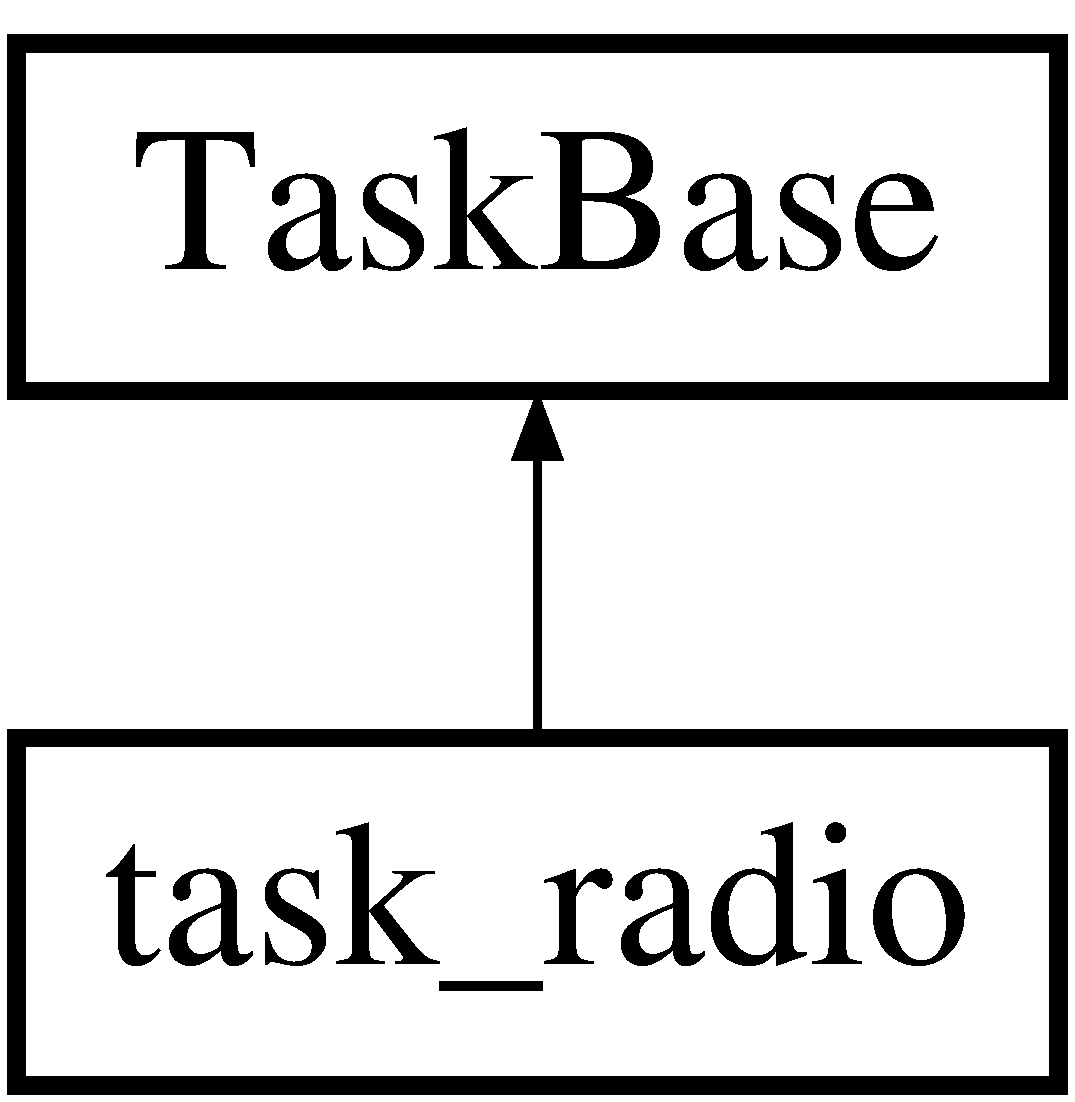
\includegraphics[height=2.000000cm]{classtask__radio}
\end{center}
\end{figure}
\subsection*{Public Member Functions}
\begin{DoxyCompactItemize}
\item 
\mbox{\hyperlink{classtask__radio_ad6d6a721a2642bb3074d682ea880aa30}{task\+\_\+radio}} (const char $\ast$, unsigned port\+B\+A\+S\+E\+\_\+\+T\+Y\+PE, size\+\_\+t, emstream $\ast$)
\item 
void \mbox{\hyperlink{classtask__radio_a4aeed57265c3fd031bd1219a9854811d}{run}} (void)
\end{DoxyCompactItemize}
\subsection*{Protected Member Functions}
\begin{DoxyCompactItemize}
\item 
void \mbox{\hyperlink{classtask__radio_ae65a87dacc155acdc221ca640a6812f8}{init\+\_\+spi}} (void)
\begin{DoxyCompactList}\small\item\em A method to initialize the S\+PI interface to the RF module. \end{DoxyCompactList}\item 
char \mbox{\hyperlink{classtask__radio_ae18b22460053f286ad2327b785cfa018}{write\+\_\+byte}} (char)
\begin{DoxyCompactList}\small\item\em A method to send a byte to the RF module. \end{DoxyCompactList}\item 
uint8\+\_\+t \mbox{\hyperlink{classtask__radio_a864714d4a62ca47b6852272d70aa0a0e}{get\+\_\+reg}} (uint8\+\_\+t)
\begin{DoxyCompactList}\small\item\em A method to get the value of a register on the RF module. \end{DoxyCompactList}\item 
uint8\+\_\+t $\ast$ \mbox{\hyperlink{classtask__radio_a06d1554c99f26f78698d156f8a729ec7}{read\+\_\+or\+\_\+write}} (uint8\+\_\+t, uint8\+\_\+t, uint8\+\_\+t $\ast$, uint8\+\_\+t)
\begin{DoxyCompactList}\small\item\em A method to write data to the RF module. \end{DoxyCompactList}\item 
void \mbox{\hyperlink{classtask__radio_ae86d2810bfbf4174f73b6c975f2deef4}{transmit}} (uint8\+\_\+t $\ast$)
\begin{DoxyCompactList}\small\item\em A method to transmit a character array with the RF module. \end{DoxyCompactList}\end{DoxyCompactItemize}


\subsection{Detailed Description}
This task is used to control the RF transciever. 

This task inherits the Task\+Base class, and is used to run as a finite state machine. It controls the actions of the RF transciever using an S\+PI interface. While this task can communicate with the RF transciever, we have not gotten the transciever to communicate with another RF module. 

Definition at line 61 of file task\+\_\+radio.\+h.



\subsection{Constructor \& Destructor Documentation}
\mbox{\Hypertarget{classtask__radio_ad6d6a721a2642bb3074d682ea880aa30}\label{classtask__radio_ad6d6a721a2642bb3074d682ea880aa30}} 
\index{task\+\_\+radio@{task\+\_\+radio}!task\+\_\+radio@{task\+\_\+radio}}
\index{task\+\_\+radio@{task\+\_\+radio}!task\+\_\+radio@{task\+\_\+radio}}
\subsubsection{\texorpdfstring{task\+\_\+radio()}{task\_radio()}}
{\footnotesize\ttfamily task\+\_\+radio\+::task\+\_\+radio (\begin{DoxyParamCaption}\item[{const char $\ast$}]{a\+\_\+name,  }\item[{unsigned port\+B\+A\+S\+E\+\_\+\+T\+Y\+PE}]{a\+\_\+priority,  }\item[{size\+\_\+t}]{a\+\_\+stack\+\_\+size,  }\item[{emstream $\ast$}]{p\+\_\+ser\+\_\+dev }\end{DoxyParamCaption})}

This constructor creates a new data acquisition task. Its main job is to call the parent class\textquotesingle{}s constructor which does most of the work. 
\begin{DoxyParams}{Parameters}
{\em a\+\_\+name} & A character string which will be the name of this task \\
\hline
{\em a\+\_\+priority} & The priority at which this task will initially run (default\+: 0) \\
\hline
{\em a\+\_\+stack\+\_\+size} & The size of this task\textquotesingle{}s stack in bytes (default\+: config\+M\+I\+N\+I\+M\+A\+L\+\_\+\+S\+T\+A\+C\+K\+\_\+\+S\+I\+ZE) \\
\hline
{\em p\+\_\+ser\+\_\+dev} & A pointer to the serial port which writes debugging info. \\
\hline
\end{DoxyParams}


Definition at line 48 of file task\+\_\+radio.\+cpp.



\subsection{Member Function Documentation}
\mbox{\Hypertarget{classtask__radio_a864714d4a62ca47b6852272d70aa0a0e}\label{classtask__radio_a864714d4a62ca47b6852272d70aa0a0e}} 
\index{task\+\_\+radio@{task\+\_\+radio}!get\+\_\+reg@{get\+\_\+reg}}
\index{get\+\_\+reg@{get\+\_\+reg}!task\+\_\+radio@{task\+\_\+radio}}
\subsubsection{\texorpdfstring{get\+\_\+reg()}{get\_reg()}}
{\footnotesize\ttfamily uint8\+\_\+t task\+\_\+radio\+::get\+\_\+reg (\begin{DoxyParamCaption}\item[{uint8\+\_\+t}]{reg }\end{DoxyParamCaption})\hspace{0.3cm}{\ttfamily [protected]}}



A method to get the value of a register on the RF module. 

This method uses the S\+PI data register on our microcontroller to send a byte of information to the RF module. 
\begin{DoxyParams}{Parameters}
{\em reg} & A uint8\+\_\+t value that corresonds to the desired register. \\
\hline
\end{DoxyParams}
\begin{DoxyReturn}{Returns}
reg The uint8\+\_\+t data that was contained in the desired register RF module. 
\end{DoxyReturn}


Definition at line 201 of file task\+\_\+radio.\+cpp.



References write\+\_\+byte().



Referenced by run().

\mbox{\Hypertarget{classtask__radio_ae65a87dacc155acdc221ca640a6812f8}\label{classtask__radio_ae65a87dacc155acdc221ca640a6812f8}} 
\index{task\+\_\+radio@{task\+\_\+radio}!init\+\_\+spi@{init\+\_\+spi}}
\index{init\+\_\+spi@{init\+\_\+spi}!task\+\_\+radio@{task\+\_\+radio}}
\subsubsection{\texorpdfstring{init\+\_\+spi()}{init\_spi()}}
{\footnotesize\ttfamily void task\+\_\+radio\+::init\+\_\+spi (\begin{DoxyParamCaption}\item[{void}]{ }\end{DoxyParamCaption})\hspace{0.3cm}{\ttfamily [protected]}}



A method to initialize the S\+PI interface to the RF module. 

This method sets the correct S\+PI pins as inputs and outputs, and sets their states so that the S\+PI interface can connect to the RF module. 

Definition at line 159 of file task\+\_\+radio.\+cpp.



Referenced by run().

\mbox{\Hypertarget{classtask__radio_a06d1554c99f26f78698d156f8a729ec7}\label{classtask__radio_a06d1554c99f26f78698d156f8a729ec7}} 
\index{task\+\_\+radio@{task\+\_\+radio}!read\+\_\+or\+\_\+write@{read\+\_\+or\+\_\+write}}
\index{read\+\_\+or\+\_\+write@{read\+\_\+or\+\_\+write}!task\+\_\+radio@{task\+\_\+radio}}
\subsubsection{\texorpdfstring{read\+\_\+or\+\_\+write()}{read\_or\_write()}}
{\footnotesize\ttfamily uint8\+\_\+t $\ast$ task\+\_\+radio\+::read\+\_\+or\+\_\+write (\begin{DoxyParamCaption}\item[{uint8\+\_\+t}]{Read\+Write,  }\item[{uint8\+\_\+t}]{reg,  }\item[{uint8\+\_\+t $\ast$}]{val,  }\item[{uint8\+\_\+t}]{ant\+Val }\end{DoxyParamCaption})\hspace{0.3cm}{\ttfamily [protected]}}



A method to write data to the RF module. 

This method uses the S\+PI data register on our microcontroller to send a byte of information to the RF module. 
\begin{DoxyParams}{Parameters}
{\em Read\+Write} & A uint8\+\_\+t character that corresponds to either a value being written to or read from the RF module. \\
\hline
{\em reg} & A uint8\+\_\+t value that corresponds to the register of the RF module that is being modified. \\
\hline
{\em val} & A pointer to the values array that are to written to the RF module. \\
\hline
{\em ant\+Val} & A uint8\+\_\+t value that signifies the number of bytes to write to the RF module. \\
\hline
\end{DoxyParams}
\begin{DoxyReturn}{Returns}
ret The array of uint8\+\_\+t$\ast$ data that was sent to the RF module. 
\end{DoxyReturn}


Definition at line 231 of file task\+\_\+radio.\+cpp.



References write\+\_\+byte().



Referenced by run(), and transmit().

\mbox{\Hypertarget{classtask__radio_a4aeed57265c3fd031bd1219a9854811d}\label{classtask__radio_a4aeed57265c3fd031bd1219a9854811d}} 
\index{task\+\_\+radio@{task\+\_\+radio}!run@{run}}
\index{run@{run}!task\+\_\+radio@{task\+\_\+radio}}
\subsubsection{\texorpdfstring{run()}{run()}}
{\footnotesize\ttfamily void task\+\_\+radio\+::run (\begin{DoxyParamCaption}\item[{void}]{ }\end{DoxyParamCaption})}

This method is called by the R\+T\+OS once to run the task loop for ever and ever.

This task handles sending messages over the transciever to the transponder 

Definition at line 64 of file task\+\_\+radio.\+cpp.



References get\+\_\+reg(), init\+\_\+spi(), p\+\_\+rf\+\_\+ping, read\+\_\+or\+\_\+write(), and transmit().

\mbox{\Hypertarget{classtask__radio_ae86d2810bfbf4174f73b6c975f2deef4}\label{classtask__radio_ae86d2810bfbf4174f73b6c975f2deef4}} 
\index{task\+\_\+radio@{task\+\_\+radio}!transmit@{transmit}}
\index{transmit@{transmit}!task\+\_\+radio@{task\+\_\+radio}}
\subsubsection{\texorpdfstring{transmit()}{transmit()}}
{\footnotesize\ttfamily void task\+\_\+radio\+::transmit (\begin{DoxyParamCaption}\item[{uint8\+\_\+t $\ast$}]{W\+\_\+buff }\end{DoxyParamCaption})\hspace{0.3cm}{\ttfamily [protected]}}



A method to transmit a character array with the RF module. 

This method uses the read\+\_\+or\+\_\+write method to transmit an array of characters using the RF module. 
\begin{DoxyParams}{Parameters}
{\em W\+\_\+buff} & A uint8\+\_\+t$\ast$ pointer to an array which is to be sent to the RF module. \\
\hline
\end{DoxyParams}


Definition at line 273 of file task\+\_\+radio.\+cpp.



References read\+\_\+or\+\_\+write().



Referenced by run().

\mbox{\Hypertarget{classtask__radio_ae18b22460053f286ad2327b785cfa018}\label{classtask__radio_ae18b22460053f286ad2327b785cfa018}} 
\index{task\+\_\+radio@{task\+\_\+radio}!write\+\_\+byte@{write\+\_\+byte}}
\index{write\+\_\+byte@{write\+\_\+byte}!task\+\_\+radio@{task\+\_\+radio}}
\subsubsection{\texorpdfstring{write\+\_\+byte()}{write\_byte()}}
{\footnotesize\ttfamily char task\+\_\+radio\+::write\+\_\+byte (\begin{DoxyParamCaption}\item[{char}]{c\+\_\+data }\end{DoxyParamCaption})\hspace{0.3cm}{\ttfamily [protected]}}



A method to send a byte to the RF module. 

This method uses the S\+PI data register on our microcontroller to send a byte of information to the RF module. 
\begin{DoxyParams}{Parameters}
{\em c\+\_\+data} & A char byte that is to be sent to the RF module. \\
\hline
\end{DoxyParams}
\begin{DoxyReturn}{Returns}
S\+P\+DR The char data that was sent to the RF module. 
\end{DoxyReturn}


Definition at line 183 of file task\+\_\+radio.\+cpp.



Referenced by get\+\_\+reg(), and read\+\_\+or\+\_\+write().



The documentation for this class was generated from the following files\+:\begin{DoxyCompactItemize}
\item 
\mbox{\hyperlink{task__radio_8h}{task\+\_\+radio.\+h}}\item 
\mbox{\hyperlink{task__radio_8cpp}{task\+\_\+radio.\+cpp}}\end{DoxyCompactItemize}

\hypertarget{classtask__steering}{}\section{task\+\_\+steering Class Reference}
\label{classtask__steering}\index{task\+\_\+steering@{task\+\_\+steering}}


This task is used to control the position of the servo.  




{\ttfamily \#include $<$task\+\_\+steering.\+h$>$}

Inheritance diagram for task\+\_\+steering\+:\begin{figure}[H]
\begin{center}
\leavevmode
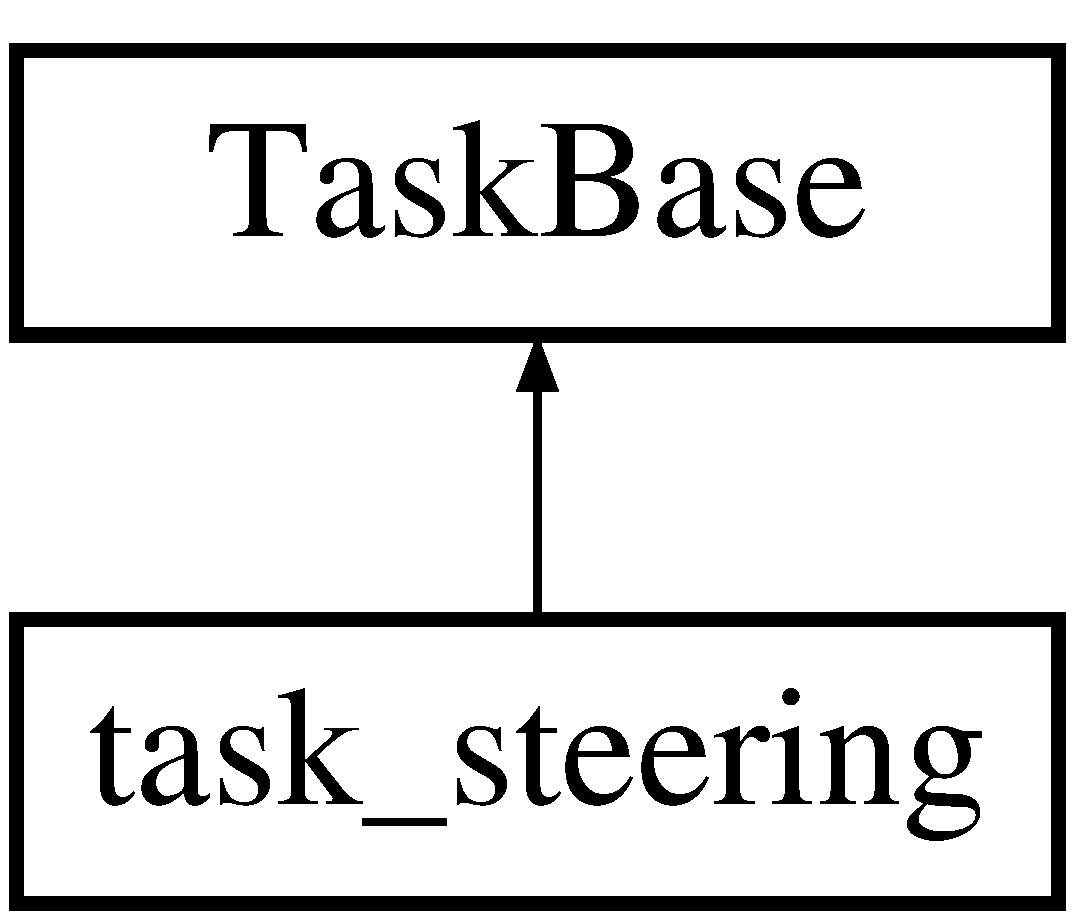
\includegraphics[height=2.000000cm]{classtask__steering}
\end{center}
\end{figure}
\subsection*{Public Member Functions}
\begin{DoxyCompactItemize}
\item 
\mbox{\hyperlink{classtask__steering_af8a9a96908212f23d97b2f859b571c4d}{task\+\_\+steering}} (const char $\ast$, unsigned port\+B\+A\+S\+E\+\_\+\+T\+Y\+PE, size\+\_\+t, emstream $\ast$)
\item 
void \mbox{\hyperlink{classtask__steering_a223e9f1d50c0c48ff5326b7ae01ae689}{run}} (void)
\begin{DoxyCompactList}\small\item\em This method is called by the R\+T\+OS once to run the task loop for ever and ever. \end{DoxyCompactList}\end{DoxyCompactItemize}
\subsection*{Protected Member Functions}
\begin{DoxyCompactItemize}
\item 
uint8\+\_\+t \mbox{\hyperlink{classtask__steering_a6f33131ca25de22a81282b1142d939b3}{calc\+\_\+pwm}} (int8\+\_\+t)
\begin{DoxyCompactList}\small\item\em This method calculates the P\+WM length to be sent to the servo timer. \end{DoxyCompactList}\end{DoxyCompactItemize}


\subsection{Detailed Description}
This task is used to control the position of the servo. 

This task inherits the Task\+Base class, and is used to run as a finite state machine. It controls the actions of the servo using a timer for P\+WM. 

Definition at line 55 of file task\+\_\+steering.\+h.



\subsection{Constructor \& Destructor Documentation}
\mbox{\Hypertarget{classtask__steering_af8a9a96908212f23d97b2f859b571c4d}\label{classtask__steering_af8a9a96908212f23d97b2f859b571c4d}} 
\index{task\+\_\+steering@{task\+\_\+steering}!task\+\_\+steering@{task\+\_\+steering}}
\index{task\+\_\+steering@{task\+\_\+steering}!task\+\_\+steering@{task\+\_\+steering}}
\subsubsection{\texorpdfstring{task\+\_\+steering()}{task\_steering()}}
{\footnotesize\ttfamily task\+\_\+steering\+::task\+\_\+steering (\begin{DoxyParamCaption}\item[{const char $\ast$}]{a\+\_\+name,  }\item[{unsigned port\+B\+A\+S\+E\+\_\+\+T\+Y\+PE}]{a\+\_\+priority,  }\item[{size\+\_\+t}]{a\+\_\+stack\+\_\+size,  }\item[{emstream $\ast$}]{p\+\_\+ser\+\_\+dev }\end{DoxyParamCaption})}

This constructor creates a task to control the servo angle. It is used to control the movement direction of the car. 
\begin{DoxyParams}{Parameters}
{\em a\+\_\+name} & A character string which will be the name of this task \\
\hline
{\em a\+\_\+priority} & The priority at which this task will initially run (default\+: 0) \\
\hline
{\em a\+\_\+stack\+\_\+size} & The size of this task\textquotesingle{}s stack in bytes (default\+: config\+M\+I\+N\+I\+M\+A\+L\+\_\+\+S\+T\+A\+C\+K\+\_\+\+S\+I\+ZE) \\
\hline
{\em p\+\_\+ser\+\_\+dev} & A pointer to the serial port which writes debugging info. \\
\hline
\end{DoxyParams}


Definition at line 46 of file task\+\_\+steering.\+cpp.



\subsection{Member Function Documentation}
\mbox{\Hypertarget{classtask__steering_a6f33131ca25de22a81282b1142d939b3}\label{classtask__steering_a6f33131ca25de22a81282b1142d939b3}} 
\index{task\+\_\+steering@{task\+\_\+steering}!calc\+\_\+pwm@{calc\+\_\+pwm}}
\index{calc\+\_\+pwm@{calc\+\_\+pwm}!task\+\_\+steering@{task\+\_\+steering}}
\subsubsection{\texorpdfstring{calc\+\_\+pwm()}{calc\_pwm()}}
{\footnotesize\ttfamily uint8\+\_\+t task\+\_\+steering\+::calc\+\_\+pwm (\begin{DoxyParamCaption}\item[{int8\+\_\+t}]{pwm }\end{DoxyParamCaption})\hspace{0.3cm}{\ttfamily [protected]}}



This method calculates the P\+WM length to be sent to the servo timer. 

This method takes a single input of the desired servo position. From this value, the timer pulse length that corresponds to this position is calculated and returned. \begin{DoxyReturn}{Returns}
pulse\+\_\+length A uint8\+\_\+t type variable that represents the counter value to be written to timer register so that the correct motor speed will be achieved. 
\end{DoxyReturn}


Definition at line 136 of file task\+\_\+steering.\+cpp.



Referenced by run().

\mbox{\Hypertarget{classtask__steering_a223e9f1d50c0c48ff5326b7ae01ae689}\label{classtask__steering_a223e9f1d50c0c48ff5326b7ae01ae689}} 
\index{task\+\_\+steering@{task\+\_\+steering}!run@{run}}
\index{run@{run}!task\+\_\+steering@{task\+\_\+steering}}
\subsubsection{\texorpdfstring{run()}{run()}}
{\footnotesize\ttfamily void task\+\_\+steering\+::run (\begin{DoxyParamCaption}\item[{void}]{ }\end{DoxyParamCaption})}



This method is called by the R\+T\+OS once to run the task loop for ever and ever. 

This method is called to run the servo control loop.

This function works within the Free\+R\+T\+OS framework. Once it is called, it loops through a switch for as long as the main program is running in a finite state machine. This task uses the shared p\+\_\+servo\+\_\+pos variable calculate and set the P\+WM signal which activates the servo. 

Definition at line 66 of file task\+\_\+steering.\+cpp.



References calc\+\_\+pwm(), and p\+\_\+servo\+\_\+pos.



The documentation for this class was generated from the following files\+:\begin{DoxyCompactItemize}
\item 
\mbox{\hyperlink{task__steering_8h}{task\+\_\+steering.\+h}}\item 
\mbox{\hyperlink{task__steering_8cpp}{task\+\_\+steering.\+cpp}}\end{DoxyCompactItemize}

\hypertarget{classtask__user}{}\section{task\+\_\+user Class Reference}
\label{classtask__user}\index{task\+\_\+user@{task\+\_\+user}}


{\ttfamily \#include $<$task\+\_\+user.\+h$>$}

Inheritance diagram for task\+\_\+user\+:\begin{figure}[H]
\begin{center}
\leavevmode
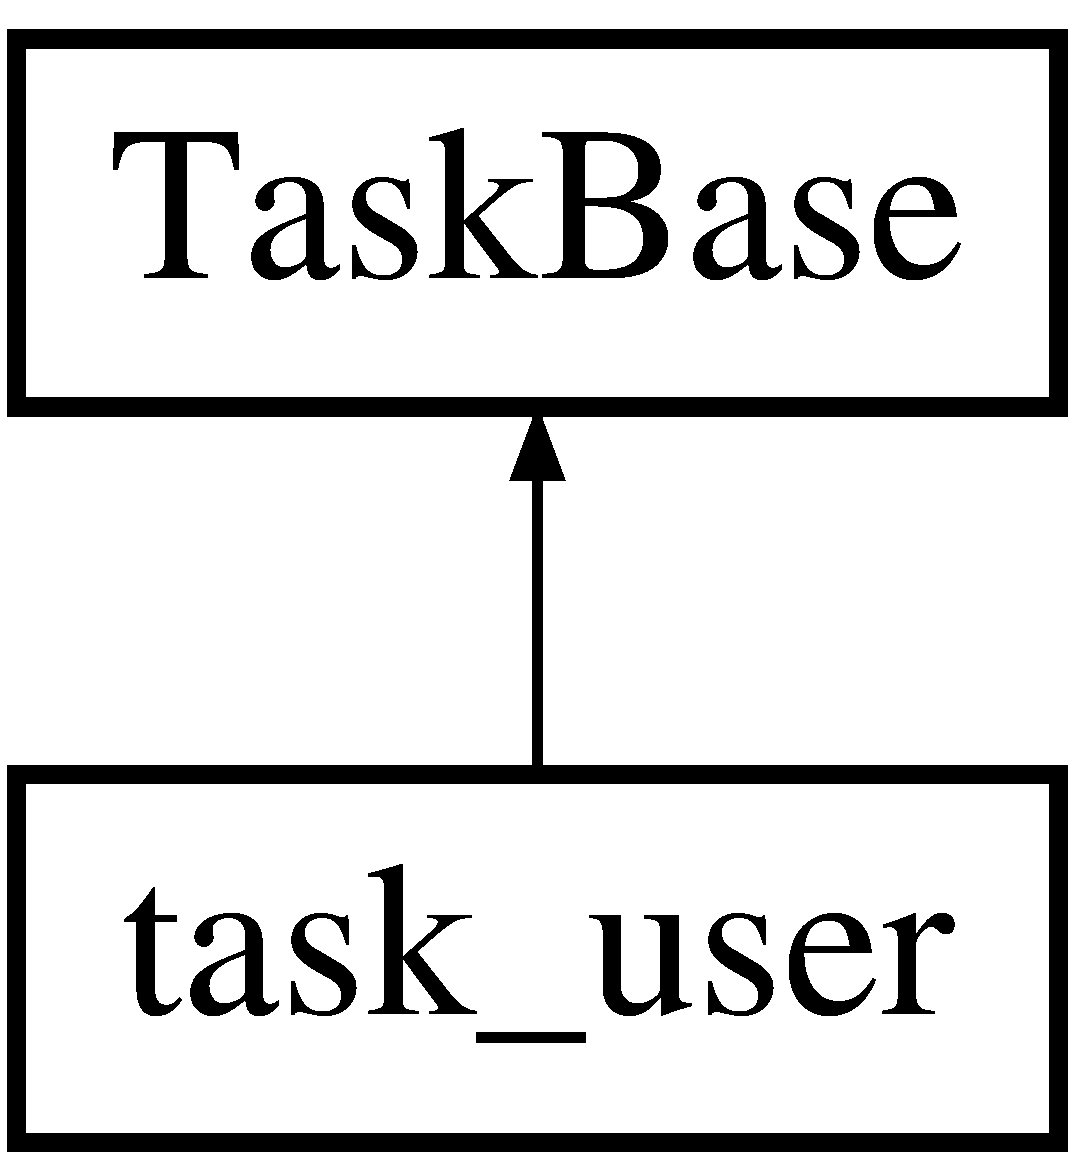
\includegraphics[height=2.000000cm]{classtask__user}
\end{center}
\end{figure}
\subsection*{Public Member Functions}
\begin{DoxyCompactItemize}
\item 
\mbox{\hyperlink{classtask__user_a3aba77563b375bb14838800608da48bc}{task\+\_\+user}} (const char $\ast$, unsigned port\+B\+A\+S\+E\+\_\+\+T\+Y\+PE, size\+\_\+t, emstream $\ast$)
\item 
void \mbox{\hyperlink{classtask__user_adca6429d57be25e8d411414fc8ad75af}{run}} (void)
\end{DoxyCompactItemize}
\subsection*{Protected Member Functions}
\begin{DoxyCompactItemize}
\item 
void \mbox{\hyperlink{classtask__user_a75475060f83bae1e44bcc8a5c34015c7}{print\+\_\+help\+\_\+message}} (void)
\item 
void \mbox{\hyperlink{classtask__user_a105bebbd9cb1031154c3dfc3662db4a0}{show\+\_\+status}} (void)
\end{DoxyCompactItemize}


\subsection{Detailed Description}
This task interacts with the user for force him/her to do what he/she is told. What a rude task this is. Then again, computers tend to be that way; if they\textquotesingle{}re polite with you, they\textquotesingle{}re probably spying on you. 

Definition at line 60 of file task\+\_\+user.\+h.



\subsection{Constructor \& Destructor Documentation}
\mbox{\Hypertarget{classtask__user_a3aba77563b375bb14838800608da48bc}\label{classtask__user_a3aba77563b375bb14838800608da48bc}} 
\index{task\+\_\+user@{task\+\_\+user}!task\+\_\+user@{task\+\_\+user}}
\index{task\+\_\+user@{task\+\_\+user}!task\+\_\+user@{task\+\_\+user}}
\subsubsection{\texorpdfstring{task\+\_\+user()}{task\_user()}}
{\footnotesize\ttfamily task\+\_\+user\+::task\+\_\+user (\begin{DoxyParamCaption}\item[{const char $\ast$}]{a\+\_\+name,  }\item[{unsigned port\+B\+A\+S\+E\+\_\+\+T\+Y\+PE}]{a\+\_\+priority,  }\item[{size\+\_\+t}]{a\+\_\+stack\+\_\+size,  }\item[{emstream $\ast$}]{p\+\_\+ser\+\_\+dev }\end{DoxyParamCaption})}

This constructor creates a new data acquisition task. Its main job is to call the parent class\textquotesingle{}s constructor which does most of the work. 
\begin{DoxyParams}{Parameters}
{\em a\+\_\+name} & A character string which will be the name of this task \\
\hline
{\em a\+\_\+priority} & The priority at which this task will initially run (default\+: 0) \\
\hline
{\em a\+\_\+stack\+\_\+size} & The size of this task\textquotesingle{}s stack in bytes (default\+: config\+M\+I\+N\+I\+M\+A\+L\+\_\+\+S\+T\+A\+C\+K\+\_\+\+S\+I\+ZE) \\
\hline
{\em p\+\_\+ser\+\_\+dev} & Pointer to a serial device (port, radio, SD card, etc.) which can be used by this task to communicate (default\+: N\+U\+LL) \\
\hline
\end{DoxyParams}


Definition at line 52 of file task\+\_\+user.\+cpp.



\subsection{Member Function Documentation}
\mbox{\Hypertarget{classtask__user_a75475060f83bae1e44bcc8a5c34015c7}\label{classtask__user_a75475060f83bae1e44bcc8a5c34015c7}} 
\index{task\+\_\+user@{task\+\_\+user}!print\+\_\+help\+\_\+message@{print\+\_\+help\+\_\+message}}
\index{print\+\_\+help\+\_\+message@{print\+\_\+help\+\_\+message}!task\+\_\+user@{task\+\_\+user}}
\subsubsection{\texorpdfstring{print\+\_\+help\+\_\+message()}{print\_help\_message()}}
{\footnotesize\ttfamily void task\+\_\+user\+::print\+\_\+help\+\_\+message (\begin{DoxyParamCaption}\item[{void}]{ }\end{DoxyParamCaption})\hspace{0.3cm}{\ttfamily [protected]}}

This method prints a simple help message. 

Definition at line 233 of file task\+\_\+user.\+cpp.



References P\+R\+O\+G\+R\+A\+M\+\_\+\+V\+E\+R\+S\+I\+ON.

\mbox{\Hypertarget{classtask__user_adca6429d57be25e8d411414fc8ad75af}\label{classtask__user_adca6429d57be25e8d411414fc8ad75af}} 
\index{task\+\_\+user@{task\+\_\+user}!run@{run}}
\index{run@{run}!task\+\_\+user@{task\+\_\+user}}
\subsubsection{\texorpdfstring{run()}{run()}}
{\footnotesize\ttfamily void task\+\_\+user\+::run (\begin{DoxyParamCaption}\item[{void}]{ }\end{DoxyParamCaption})}

This method is called by the R\+T\+OS once to run the task loop for ever and ever.

This task interacts with the user for force him/her to do what he/she is told. It is just following the modern government model of \char`\"{}\+This is the land of the free...
free to do exactly what you\textquotesingle{}re told.\char`\"{} 

Definition at line 70 of file task\+\_\+user.\+cpp.

\mbox{\Hypertarget{classtask__user_a105bebbd9cb1031154c3dfc3662db4a0}\label{classtask__user_a105bebbd9cb1031154c3dfc3662db4a0}} 
\index{task\+\_\+user@{task\+\_\+user}!show\+\_\+status@{show\+\_\+status}}
\index{show\+\_\+status@{show\+\_\+status}!task\+\_\+user@{task\+\_\+user}}
\subsubsection{\texorpdfstring{show\+\_\+status()}{show\_status()}}
{\footnotesize\ttfamily void task\+\_\+user\+::show\+\_\+status (\begin{DoxyParamCaption}\item[{void}]{ }\end{DoxyParamCaption})\hspace{0.3cm}{\ttfamily [protected]}}

This method displays information about the status of the system, including the following\+: \begin{DoxyItemize}
\item The name and version of the program \item The name, status, priority, and free stack space of each task \item Processor cycles used by each task \item Amount of heap space free and setting of R\+T\+OS tick timer \end{DoxyItemize}


Definition at line 258 of file task\+\_\+user.\+cpp.



References P\+R\+O\+G\+R\+A\+M\+\_\+\+V\+E\+R\+S\+I\+ON.



The documentation for this class was generated from the following files\+:\begin{DoxyCompactItemize}
\item 
\mbox{\hyperlink{task__user_8h}{task\+\_\+user.\+h}}\item 
\mbox{\hyperlink{task__user_8cpp}{task\+\_\+user.\+cpp}}\end{DoxyCompactItemize}

\hypertarget{classtask__USR1}{}\section{task\+\_\+\+U\+S\+R1 Class Reference}
\label{classtask__USR1}\index{task\+\_\+\+U\+S\+R1@{task\+\_\+\+U\+S\+R1}}


This task is used to run the distance sensor.  




{\ttfamily \#include $<$task\+\_\+\+U\+S\+R1.\+h$>$}

Inheritance diagram for task\+\_\+\+U\+S\+R1\+:\begin{figure}[H]
\begin{center}
\leavevmode
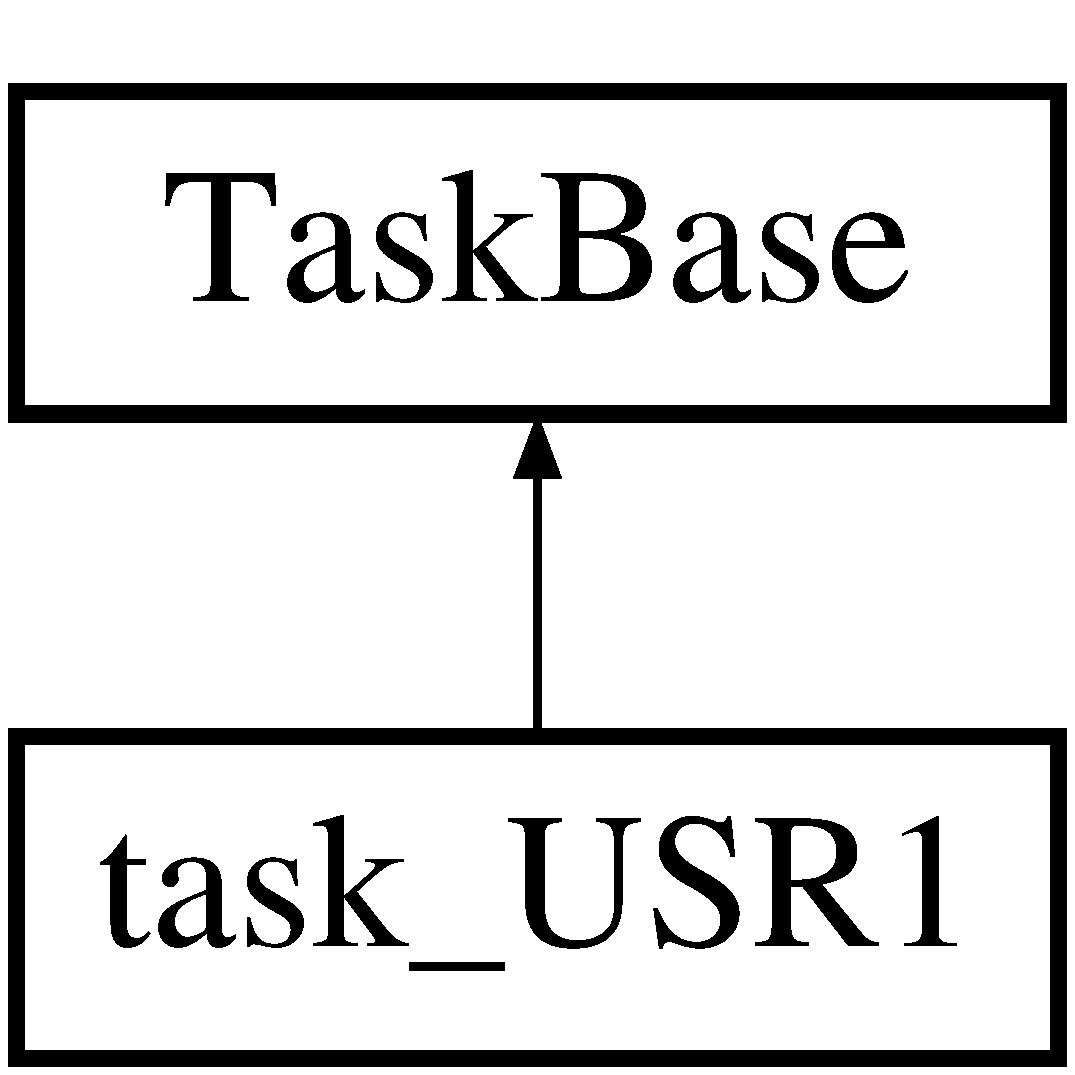
\includegraphics[height=2.000000cm]{classtask__USR1}
\end{center}
\end{figure}
\subsection*{Public Member Functions}
\begin{DoxyCompactItemize}
\item 
\mbox{\hyperlink{classtask__USR1_a09b56d4b1411901f63f762174266ecfa}{task\+\_\+\+U\+S\+R1}} (const char $\ast$, unsigned port\+B\+A\+S\+E\+\_\+\+T\+Y\+PE, size\+\_\+t, emstream $\ast$)
\item 
void \mbox{\hyperlink{classtask__USR1_a95b84a7b7f293a56470b74eb541fe346}{run}} (void)
\begin{DoxyCompactList}\small\item\em This method is called to run the Ultrasonic distance sensor task. \end{DoxyCompactList}\end{DoxyCompactItemize}
\subsection*{Protected Attributes}
\begin{DoxyCompactItemize}
\item 
\mbox{\Hypertarget{classtask__USR1_a306766d3d24e1682f19c2e5ee4c3d8ce}\label{classtask__USR1_a306766d3d24e1682f19c2e5ee4c3d8ce}} 
uint8\+\_\+t \mbox{\hyperlink{classtask__USR1_a306766d3d24e1682f19c2e5ee4c3d8ce}{E\+C\+HO}}
\begin{DoxyCompactList}\small\item\em This variable is used to detect whether the Trigger pin on the distance sensor is set high or low. \end{DoxyCompactList}\end{DoxyCompactItemize}


\subsection{Detailed Description}
This task is used to run the distance sensor. 

This task inherits the Task\+Base class, and is used to run as a finite state machine. It runs the distance sensor by toggling the trigger pin, and records E\+C\+HO pulse width using input capture interrupts 

Definition at line 51 of file task\+\_\+\+U\+S\+R1.\+h.



\subsection{Constructor \& Destructor Documentation}
\mbox{\Hypertarget{classtask__USR1_a09b56d4b1411901f63f762174266ecfa}\label{classtask__USR1_a09b56d4b1411901f63f762174266ecfa}} 
\index{task\+\_\+\+U\+S\+R1@{task\+\_\+\+U\+S\+R1}!task\+\_\+\+U\+S\+R1@{task\+\_\+\+U\+S\+R1}}
\index{task\+\_\+\+U\+S\+R1@{task\+\_\+\+U\+S\+R1}!task\+\_\+\+U\+S\+R1@{task\+\_\+\+U\+S\+R1}}
\subsubsection{\texorpdfstring{task\+\_\+\+U\+S\+R1()}{task\_USR1()}}
{\footnotesize\ttfamily task\+\_\+\+U\+S\+R1\+::task\+\_\+\+U\+S\+R1 (\begin{DoxyParamCaption}\item[{const char $\ast$}]{a\+\_\+name,  }\item[{unsigned port\+B\+A\+S\+E\+\_\+\+T\+Y\+PE}]{a\+\_\+priority,  }\item[{size\+\_\+t}]{a\+\_\+stack\+\_\+size,  }\item[{emstream $\ast$}]{p\+\_\+ser\+\_\+dev }\end{DoxyParamCaption})}

This constructor creates a new data acquisition task. Its main job is to call the parent class\textquotesingle{}s constructor which does most of the work. 
\begin{DoxyParams}{Parameters}
{\em a\+\_\+name} & A character string which will be the name of this task \\
\hline
{\em a\+\_\+priority} & The priority at which this task will initially run (default\+: 0) \\
\hline
{\em a\+\_\+stack\+\_\+size} & The size of this task\textquotesingle{}s stack in bytes (default\+: config\+M\+I\+N\+I\+M\+A\+L\+\_\+\+S\+T\+A\+C\+K\+\_\+\+S\+I\+ZE) \\
\hline
{\em p\+\_\+ser\+\_\+dev} & Pointer to a serial device (port, radio, SD card, etc.) which can be used by this task to communicate (default\+: N\+U\+LL) \\
\hline
\end{DoxyParams}


Definition at line 50 of file task\+\_\+\+U\+S\+R1.\+cpp.



\subsection{Member Function Documentation}
\mbox{\Hypertarget{classtask__USR1_a95b84a7b7f293a56470b74eb541fe346}\label{classtask__USR1_a95b84a7b7f293a56470b74eb541fe346}} 
\index{task\+\_\+\+U\+S\+R1@{task\+\_\+\+U\+S\+R1}!run@{run}}
\index{run@{run}!task\+\_\+\+U\+S\+R1@{task\+\_\+\+U\+S\+R1}}
\subsubsection{\texorpdfstring{run()}{run()}}
{\footnotesize\ttfamily void task\+\_\+\+U\+S\+R1\+::run (\begin{DoxyParamCaption}\item[{void}]{ }\end{DoxyParamCaption})}



This method is called to run the Ultrasonic distance sensor task. 

This method is called by the R\+T\+OS once to run the task loop for ever and ever.

This function works within the Free\+R\+T\+OS framework. Once it is called, it initializes necessary pins, and sets up input capture interrupts to measure the E\+C\+HO pulse from the sensor.\+It also cotinually toggles the trigger pin such that the sensor continually sends pulses for object detection. 

Definition at line 72 of file task\+\_\+\+U\+S\+R1.\+cpp.



References E\+C\+HO, edge\+\_\+1, and width\+\_\+1.



The documentation for this class was generated from the following files\+:\begin{DoxyCompactItemize}
\item 
\mbox{\hyperlink{task__USR1_8h}{task\+\_\+\+U\+S\+R1.\+h}}\item 
\mbox{\hyperlink{task__USR1_8cpp}{task\+\_\+\+U\+S\+R1.\+cpp}}\end{DoxyCompactItemize}

\chapter{File Documentation}
\hypertarget{main_8cpp}{}\section{main.\+cpp File Reference}
\label{main_8cpp}\index{main.\+cpp@{main.\+cpp}}
{\ttfamily \#include $<$stdlib.\+h$>$}\newline
{\ttfamily \#include $<$avr/io.\+h$>$}\newline
{\ttfamily \#include $<$avr/wdt.\+h$>$}\newline
{\ttfamily \#include $<$string.\+h$>$}\newline
{\ttfamily \#include $<$avr/interrupt.\+h$>$}\newline
{\ttfamily \#include \char`\"{}Free\+R\+T\+O\+S.\+h\char`\"{}}\newline
{\ttfamily \#include \char`\"{}task.\+h\char`\"{}}\newline
{\ttfamily \#include \char`\"{}queue.\+h\char`\"{}}\newline
{\ttfamily \#include \char`\"{}croutine.\+h\char`\"{}}\newline
{\ttfamily \#include \char`\"{}rs232int.\+h\char`\"{}}\newline
{\ttfamily \#include \char`\"{}time\+\_\+stamp.\+h\char`\"{}}\newline
{\ttfamily \#include \char`\"{}taskbase.\+h\char`\"{}}\newline
{\ttfamily \#include \char`\"{}textqueue.\+h\char`\"{}}\newline
{\ttfamily \#include \char`\"{}taskqueue.\+h\char`\"{}}\newline
{\ttfamily \#include \char`\"{}taskshare.\+h\char`\"{}}\newline
{\ttfamily \#include \char`\"{}shares.\+h\char`\"{}}\newline
{\ttfamily \#include \char`\"{}task\+\_\+user.\+h\char`\"{}}\newline
{\ttfamily \#include \char`\"{}task\+\_\+steering.\+h\char`\"{}}\newline
{\ttfamily \#include \char`\"{}task\+\_\+motor.\+h\char`\"{}}\newline
{\ttfamily \#include \char`\"{}task\+\_\+car\+\_\+control.\+h\char`\"{}}\newline
{\ttfamily \#include \char`\"{}task\+\_\+radio.\+h\char`\"{}}\newline
{\ttfamily \#include \char`\"{}task\+\_\+\+U\+S\+R1.\+h\char`\"{}}\newline
\subsection*{Functions}
\begin{DoxyCompactItemize}
\item 
int \mbox{\hyperlink{main_8cpp_a840291bc02cba5474a4cb46a9b9566fe}{main}} (void)
\item 
\mbox{\hyperlink{main_8cpp_afdd244607cefccfe77024721d1ab9622}{I\+SR}} (T\+I\+M\+E\+R3\+\_\+\+C\+A\+P\+T\+\_\+vect)
\begin{DoxyCompactList}\small\item\em An I\+SR routine to determine pulse width received from distance sensor. \end{DoxyCompactList}\end{DoxyCompactItemize}
\subsection*{Variables}
\begin{DoxyCompactItemize}
\item 
Text\+Queue $\ast$ \mbox{\hyperlink{main_8cpp_acd99bf5d187d4809af2f460a5415e904}{p\+\_\+print\+\_\+ser\+\_\+queue}}
\begin{DoxyCompactList}\small\item\em A queue to print data to a serial port in a task friendly way. \end{DoxyCompactList}\item 
Task\+Share$<$ int8\+\_\+t $>$ $\ast$ \mbox{\hyperlink{main_8cpp_a658458b35e40d0a0ba7b27a99667273d}{p\+\_\+servo\+\_\+pos}}
\begin{DoxyCompactList}\small\item\em A pointer to a variable that controls the servo position. \end{DoxyCompactList}\item 
Task\+Share$<$ int8\+\_\+t $>$ $\ast$ \mbox{\hyperlink{main_8cpp_a377a9ec5b3493875d102b708b87c7b1f}{p\+\_\+motor\+\_\+vel}}
\begin{DoxyCompactList}\small\item\em A pointer to a variable that controls the motor velocity. \end{DoxyCompactList}\item 
Task\+Share$<$ int8\+\_\+t $>$ $\ast$ \mbox{\hyperlink{main_8cpp_aaba85f0f59ab3fbdbbb3e9fee5f48795}{p\+\_\+enc\+\_\+read}}
\begin{DoxyCompactList}\small\item\em A pointer to a variable that represents the encoder ticks per second. \end{DoxyCompactList}\item 
Task\+Share$<$ bool $>$ $\ast$ \mbox{\hyperlink{main_8cpp_a188eb21a8430d67a13e1a49e8a4247bc}{p\+\_\+rf\+\_\+ping}}
\begin{DoxyCompactList}\small\item\em A pointer to a variable that tells the RF module to ping the transponder. \end{DoxyCompactList}\item 
Task\+Share$<$ uint8\+\_\+t $>$ $\ast$ \mbox{\hyperlink{main_8cpp_a417763188f0e12c3bc2627b0783cf562}{p\+\_\+drive\+\_\+state}}
\begin{DoxyCompactList}\small\item\em A pointer to a variable that controls the drive state. \end{DoxyCompactList}\item 
Task\+Share$<$ int8\+\_\+t $>$ $\ast$ \mbox{\hyperlink{main_8cpp_ad2bc6c6fe7bf518436a70d7f9384aab2}{edge\+\_\+1}}
\begin{DoxyCompactList}\small\item\em A pointer to a variable that represents the edge change for the I\+SR. \end{DoxyCompactList}\item 
Task\+Share$<$ uint16\+\_\+t $>$ $\ast$ \mbox{\hyperlink{main_8cpp_ad554ea3ddab2e460573f8c5ee31eb44d}{width\+\_\+1}}
\begin{DoxyCompactList}\small\item\em A pointer to the pulse width value of the distance sensor E\+C\+HO pin. \end{DoxyCompactList}\end{DoxyCompactItemize}


\subsection{Detailed Description}
This file contains the \mbox{\hyperlink{main_8cpp_a840291bc02cba5474a4cb46a9b9566fe}{main()}} code for a multi-\/task program run under the Free\+R\+T\+OS framework.

Revisions\+: \begin{DoxyItemize}
\item 11-\/29-\/2018 KM file created to setup the task state-\/machine. \item 12-\/4-\/2018 KM added all tasks to state machine. \item 12-\/9-\/2018 KM last planned edit.\end{DoxyItemize}
License\+: This code is based on Prof. JR Ridgely\textquotesingle{}s Free\+R\+T\+OS C\+PP example code. The Free\+R\+T\+OS framework is used, but the tasks are a product of our 507 group. Since the original code used the L\+G\+PL, our code will also use the L\+G\+PL. T\+H\+IS S\+O\+F\+T\+W\+A\+RE IS P\+R\+O\+V\+I\+D\+ED BY T\+HE C\+O\+P\+Y\+R\+I\+G\+HT H\+O\+L\+D\+E\+RS A\+ND C\+O\+N\+T\+R\+I\+B\+U\+T\+O\+RS \char`\"{}\+A\+S I\+S\char`\"{} A\+ND A\+NY E\+X\+P\+R\+E\+SS OR I\+M\+P\+L\+I\+ED W\+A\+R\+R\+A\+N\+T\+I\+ES, I\+N\+C\+L\+U\+D\+I\+NG, B\+UT N\+OT L\+I\+M\+I\+T\+ED TO, T\+HE I\+M\+P\+L\+I\+ED W\+A\+R\+R\+A\+N\+T\+I\+ES OF M\+E\+R\+C\+H\+A\+N\+T\+A\+B\+I\+L\+I\+TY A\+ND F\+I\+T\+N\+E\+SS F\+OR A P\+A\+R\+T\+I\+C\+U\+L\+AR P\+U\+R\+P\+O\+SE A\+RE D\+I\+S\+C\+L\+A\+I\+M\+ED. IN NO E\+V\+E\+NT S\+H\+A\+LL T\+HE C\+O\+P\+Y\+R\+I\+G\+HT O\+W\+N\+ER OR C\+O\+N\+T\+R\+I\+B\+U\+T\+O\+RS BE L\+I\+A\+B\+LE F\+OR A\+NY D\+I\+R\+E\+CT, I\+N\+D\+I\+R\+E\+CT, I\+N\+C\+I\+D\+E\+N\+T\+AL, S\+P\+E\+C\+I\+AL, E\+X\+E\+M\+P\+L\+A\+RY, OR C\+O\+N\+S\+E\+Q\+U\+E\+N-\/ T\+I\+AL D\+A\+M\+A\+G\+ES (I\+N\+C\+L\+U\+D\+I\+NG, B\+UT N\+OT L\+I\+M\+I\+T\+ED TO, P\+R\+O\+C\+U\+R\+E\+M\+E\+NT OF S\+U\+B\+S\+T\+I\+T\+U\+TE G\+O\+O\+DS OR S\+E\+R\+V\+I\+C\+ES; L\+O\+SS OF U\+SE, D\+A\+TA, OR P\+R\+O\+F\+I\+TS; OR B\+U\+S\+I\+N\+E\+SS I\+N\+T\+E\+R\+R\+U\+P\+T\+I\+ON) H\+O\+W\+E\+V\+ER C\+A\+U\+S\+ED A\+ND ON A\+NY T\+H\+E\+O\+RY OF L\+I\+A\+B\+I\+L\+I\+TY, W\+H\+E\+T\+H\+ER IN C\+O\+N\+T\+R\+A\+CT, S\+T\+R\+I\+CT L\+I\+A\+B\+I\+L\+I\+TY, OR T\+O\+RT (I\+N\+C\+L\+U\+D\+I\+NG N\+E\+G\+L\+I\+G\+E\+N\+CE OR O\+T\+H\+E\+R\+W\+I\+SE) A\+R\+I\+S\+I\+NG IN A\+NY W\+AY O\+UT OF T\+HE U\+SE OF T\+H\+IS S\+O\+F\+T\+W\+A\+RE, E\+V\+EN IF A\+D\+V\+I\+S\+ED OF T\+HE P\+O\+S\+S\+I\+B\+I\+L\+I\+TY OF S\+U\+CH D\+A\+M\+A\+GE. 

\subsection{Function Documentation}
\mbox{\Hypertarget{main_8cpp_afdd244607cefccfe77024721d1ab9622}\label{main_8cpp_afdd244607cefccfe77024721d1ab9622}} 
\index{main.\+cpp@{main.\+cpp}!I\+SR@{I\+SR}}
\index{I\+SR@{I\+SR}!main.\+cpp@{main.\+cpp}}
\subsubsection{\texorpdfstring{I\+S\+R()}{ISR()}}
{\footnotesize\ttfamily I\+SR (\begin{DoxyParamCaption}\item[{T\+I\+M\+E\+R3\+\_\+\+C\+A\+P\+T\+\_\+vect}]{ }\end{DoxyParamCaption})}



An I\+SR routine to determine pulse width received from distance sensor. 

This routine toggles between rising and falling edge input capture to measure pulse width, and stores the value in a global variable. 

Definition at line 204 of file main.\+cpp.



References edge\+\_\+1, and width\+\_\+1.

\mbox{\Hypertarget{main_8cpp_a840291bc02cba5474a4cb46a9b9566fe}\label{main_8cpp_a840291bc02cba5474a4cb46a9b9566fe}} 
\index{main.\+cpp@{main.\+cpp}!main@{main}}
\index{main@{main}!main.\+cpp@{main.\+cpp}}
\subsubsection{\texorpdfstring{main()}{main()}}
{\footnotesize\ttfamily int main (\begin{DoxyParamCaption}\item[{void}]{ }\end{DoxyParamCaption})}

The main function sets up the R\+T\+OS. Some test tasks are created. Then the scheduler is started up; the scheduler runs until power is turned off or there\textquotesingle{}s a reset. \begin{DoxyReturn}{Returns}
This is a real-\/time microcontroller program which doesn\textquotesingle{}t return. Ever. 
\end{DoxyReturn}


Definition at line 124 of file main.\+cpp.



References edge\+\_\+1, p\+\_\+drive\+\_\+state, p\+\_\+enc\+\_\+read, p\+\_\+motor\+\_\+vel, p\+\_\+print\+\_\+ser\+\_\+queue, p\+\_\+rf\+\_\+ping, p\+\_\+servo\+\_\+pos, and width\+\_\+1.



\subsection{Variable Documentation}
\mbox{\Hypertarget{main_8cpp_ad2bc6c6fe7bf518436a70d7f9384aab2}\label{main_8cpp_ad2bc6c6fe7bf518436a70d7f9384aab2}} 
\index{main.\+cpp@{main.\+cpp}!edge\+\_\+1@{edge\+\_\+1}}
\index{edge\+\_\+1@{edge\+\_\+1}!main.\+cpp@{main.\+cpp}}
\subsubsection{\texorpdfstring{edge\+\_\+1}{edge\_1}}
{\footnotesize\ttfamily Task\+Share$<$int8\+\_\+t$>$$\ast$ edge\+\_\+1}



A pointer to a variable that represents the edge change for the I\+SR. 

edge\+\_\+1 A pointer to a int8\+\_\+t variable that stores which edge is active so that the I\+SR can return the pulse width properly. 

Definition at line 108 of file main.\+cpp.



Referenced by I\+S\+R(), main(), and task\+\_\+\+U\+S\+R1\+::run().

\mbox{\Hypertarget{main_8cpp_a417763188f0e12c3bc2627b0783cf562}\label{main_8cpp_a417763188f0e12c3bc2627b0783cf562}} 
\index{main.\+cpp@{main.\+cpp}!p\+\_\+drive\+\_\+state@{p\+\_\+drive\+\_\+state}}
\index{p\+\_\+drive\+\_\+state@{p\+\_\+drive\+\_\+state}!main.\+cpp@{main.\+cpp}}
\subsubsection{\texorpdfstring{p\+\_\+drive\+\_\+state}{p\_drive\_state}}
{\footnotesize\ttfamily Task\+Share$<$uint8\+\_\+t$>$$\ast$ p\+\_\+drive\+\_\+state}



A pointer to a variable that controls the drive state. 

p\+\_\+drive\+\_\+state A pointer to a uint8\+\_\+t Task\+Share variable that tells the car control task which state to go into. This variable is set by the user interface task and read by the car control task. 

Definition at line 102 of file main.\+cpp.



Referenced by main(), task\+\_\+car\+\_\+control\+::run(), and task\+\_\+user\+::run().

\mbox{\Hypertarget{main_8cpp_aaba85f0f59ab3fbdbbb3e9fee5f48795}\label{main_8cpp_aaba85f0f59ab3fbdbbb3e9fee5f48795}} 
\index{main.\+cpp@{main.\+cpp}!p\+\_\+enc\+\_\+read@{p\+\_\+enc\+\_\+read}}
\index{p\+\_\+enc\+\_\+read@{p\+\_\+enc\+\_\+read}!main.\+cpp@{main.\+cpp}}
\subsubsection{\texorpdfstring{p\+\_\+enc\+\_\+read}{p\_enc\_read}}
{\footnotesize\ttfamily Task\+Share$<$int8\+\_\+t$>$$\ast$ p\+\_\+enc\+\_\+read}



A pointer to a variable that represents the encoder ticks per second. 

p\+\_\+enc\+\_\+read A pointer to an int8\+\_\+t Task\+Share variable that represents the encoder ticks per second. This variable is set by the encoder read task, but is not fully implemented. 

Definition at line 88 of file main.\+cpp.



Referenced by main().

\mbox{\Hypertarget{main_8cpp_a377a9ec5b3493875d102b708b87c7b1f}\label{main_8cpp_a377a9ec5b3493875d102b708b87c7b1f}} 
\index{main.\+cpp@{main.\+cpp}!p\+\_\+motor\+\_\+vel@{p\+\_\+motor\+\_\+vel}}
\index{p\+\_\+motor\+\_\+vel@{p\+\_\+motor\+\_\+vel}!main.\+cpp@{main.\+cpp}}
\subsubsection{\texorpdfstring{p\+\_\+motor\+\_\+vel}{p\_motor\_vel}}
{\footnotesize\ttfamily Task\+Share$<$int8\+\_\+t$>$$\ast$ p\+\_\+motor\+\_\+vel}



A pointer to a variable that controls the motor velocity. 

p\+\_\+motor\+\_\+vel A pointer to an int8\+\_\+t Task\+Share variable that can control the velocity of the motor. This variable is set by the car control task and read by the servo task. 

Definition at line 81 of file main.\+cpp.



Referenced by main(), task\+\_\+car\+\_\+control\+::run(), and task\+\_\+motor\+::run().

\mbox{\Hypertarget{main_8cpp_acd99bf5d187d4809af2f460a5415e904}\label{main_8cpp_acd99bf5d187d4809af2f460a5415e904}} 
\index{main.\+cpp@{main.\+cpp}!p\+\_\+print\+\_\+ser\+\_\+queue@{p\+\_\+print\+\_\+ser\+\_\+queue}}
\index{p\+\_\+print\+\_\+ser\+\_\+queue@{p\+\_\+print\+\_\+ser\+\_\+queue}!main.\+cpp@{main.\+cpp}}
\subsubsection{\texorpdfstring{p\+\_\+print\+\_\+ser\+\_\+queue}{p\_print\_ser\_queue}}
{\footnotesize\ttfamily Text\+Queue$\ast$ p\+\_\+print\+\_\+ser\+\_\+queue}



A queue to print data to a serial port in a task friendly way. 

p\+\_\+ser\+\_\+print\+\_\+queue A pointer to a Text\+Queue serial queue object that can print data without interrupting task timing. This is utilized to by various tasks, but most importantly the user interface task. 

Definition at line 67 of file main.\+cpp.



Referenced by main(), and task\+\_\+user\+::run().

\mbox{\Hypertarget{main_8cpp_a188eb21a8430d67a13e1a49e8a4247bc}\label{main_8cpp_a188eb21a8430d67a13e1a49e8a4247bc}} 
\index{main.\+cpp@{main.\+cpp}!p\+\_\+rf\+\_\+ping@{p\+\_\+rf\+\_\+ping}}
\index{p\+\_\+rf\+\_\+ping@{p\+\_\+rf\+\_\+ping}!main.\+cpp@{main.\+cpp}}
\subsubsection{\texorpdfstring{p\+\_\+rf\+\_\+ping}{p\_rf\_ping}}
{\footnotesize\ttfamily Task\+Share$<$bool$>$$\ast$ p\+\_\+rf\+\_\+ping}



A pointer to a variable that tells the RF module to ping the transponder. 

p\+\_\+rf\+\_\+ping A pointer to a bool Task\+Share variable that tells the RF module to send a ping signal to the transciever. This variable is set by the user interface task and read by the RF module task. 

Definition at line 95 of file main.\+cpp.



Referenced by main(), task\+\_\+user\+::run(), and task\+\_\+radio\+::run().

\mbox{\Hypertarget{main_8cpp_a658458b35e40d0a0ba7b27a99667273d}\label{main_8cpp_a658458b35e40d0a0ba7b27a99667273d}} 
\index{main.\+cpp@{main.\+cpp}!p\+\_\+servo\+\_\+pos@{p\+\_\+servo\+\_\+pos}}
\index{p\+\_\+servo\+\_\+pos@{p\+\_\+servo\+\_\+pos}!main.\+cpp@{main.\+cpp}}
\subsubsection{\texorpdfstring{p\+\_\+servo\+\_\+pos}{p\_servo\_pos}}
{\footnotesize\ttfamily Task\+Share$<$int8\+\_\+t$>$$\ast$ p\+\_\+servo\+\_\+pos}



A pointer to a variable that controls the servo position. 

p\+\_\+motor\+\_\+vel A pointer to an int8\+\_\+t Task\+Share variable that can control the position of the servo. This variable is set by the car control task and read by the servo task. 

Definition at line 74 of file main.\+cpp.



Referenced by main(), task\+\_\+steering\+::run(), and task\+\_\+car\+\_\+control\+::run().

\mbox{\Hypertarget{main_8cpp_ad554ea3ddab2e460573f8c5ee31eb44d}\label{main_8cpp_ad554ea3ddab2e460573f8c5ee31eb44d}} 
\index{main.\+cpp@{main.\+cpp}!width\+\_\+1@{width\+\_\+1}}
\index{width\+\_\+1@{width\+\_\+1}!main.\+cpp@{main.\+cpp}}
\subsubsection{\texorpdfstring{width\+\_\+1}{width\_1}}
{\footnotesize\ttfamily Task\+Share$<$uint16\+\_\+t$>$$\ast$ width\+\_\+1}



A pointer to the pulse width value of the distance sensor E\+C\+HO pin. 

width\+\_\+1 A pointer to the uint16\+\_\+t variable that represents the width of the E\+C\+HO pulse for distance sensing. This variable is set in the distance sensor I\+SR. 

Definition at line 114 of file main.\+cpp.



Referenced by I\+S\+R(), main(), task\+\_\+\+U\+S\+R1\+::run(), and task\+\_\+car\+\_\+control\+::run().


\hypertarget{shares_8h}{}\section{shares.\+h File Reference}
\label{shares_8h}\index{shares.\+h@{shares.\+h}}
\subsection*{Variables}
\begin{DoxyCompactItemize}
\item 
\mbox{\Hypertarget{shares_8h_acd99bf5d187d4809af2f460a5415e904}\label{shares_8h_acd99bf5d187d4809af2f460a5415e904}} 
Text\+Queue $\ast$ {\bfseries p\+\_\+print\+\_\+ser\+\_\+queue}
\item 
\mbox{\Hypertarget{shares_8h_a377a9ec5b3493875d102b708b87c7b1f}\label{shares_8h_a377a9ec5b3493875d102b708b87c7b1f}} 
Task\+Share$<$ int8\+\_\+t $>$ $\ast$ {\bfseries p\+\_\+motor\+\_\+vel}
\item 
\mbox{\Hypertarget{shares_8h_a658458b35e40d0a0ba7b27a99667273d}\label{shares_8h_a658458b35e40d0a0ba7b27a99667273d}} 
Task\+Share$<$ int8\+\_\+t $>$ $\ast$ {\bfseries p\+\_\+servo\+\_\+pos}
\item 
\mbox{\Hypertarget{shares_8h_aaba85f0f59ab3fbdbbb3e9fee5f48795}\label{shares_8h_aaba85f0f59ab3fbdbbb3e9fee5f48795}} 
Task\+Share$<$ int8\+\_\+t $>$ $\ast$ {\bfseries p\+\_\+enc\+\_\+read}
\item 
\mbox{\Hypertarget{shares_8h_a188eb21a8430d67a13e1a49e8a4247bc}\label{shares_8h_a188eb21a8430d67a13e1a49e8a4247bc}} 
Task\+Share$<$ bool $>$ $\ast$ {\bfseries p\+\_\+rf\+\_\+ping}
\item 
\mbox{\Hypertarget{shares_8h_a417763188f0e12c3bc2627b0783cf562}\label{shares_8h_a417763188f0e12c3bc2627b0783cf562}} 
Task\+Share$<$ uint8\+\_\+t $>$ $\ast$ {\bfseries p\+\_\+drive\+\_\+state}
\item 
\mbox{\Hypertarget{shares_8h_ad2bc6c6fe7bf518436a70d7f9384aab2}\label{shares_8h_ad2bc6c6fe7bf518436a70d7f9384aab2}} 
Task\+Share$<$ int8\+\_\+t $>$ $\ast$ {\bfseries edge\+\_\+1}
\item 
\mbox{\Hypertarget{shares_8h_ad554ea3ddab2e460573f8c5ee31eb44d}\label{shares_8h_ad554ea3ddab2e460573f8c5ee31eb44d}} 
Task\+Share$<$ uint16\+\_\+t $>$ $\ast$ {\bfseries width\+\_\+1}
\end{DoxyCompactItemize}


\subsection{Detailed Description}
This file contains extern declarations for queues and other inter-\/task data communication objects for

Revisions\+: \begin{DoxyItemize}
\item 11-\/29-\/2018 KM file created to allow all tasks to access shared data.\end{DoxyItemize}
License\+: This code is based on Prof. JR Ridgely\textquotesingle{}s Free\+R\+T\+OS C\+PP example code. The Free\+R\+T\+OS framework is used, but the tasks are a product of our 507 group. Since the original code used the L\+G\+PL, our code will also use the L\+G\+PL. T\+H\+IS S\+O\+F\+T\+W\+A\+RE IS P\+R\+O\+V\+I\+D\+ED BY T\+HE C\+O\+P\+Y\+R\+I\+G\+HT H\+O\+L\+D\+E\+RS A\+ND C\+O\+N\+T\+R\+I\+B\+U\+T\+O\+RS \char`\"{}\+A\+S I\+S\char`\"{} A\+ND A\+NY E\+X\+P\+R\+E\+SS OR I\+M\+P\+L\+I\+ED W\+A\+R\+R\+A\+N\+T\+I\+ES, I\+N\+C\+L\+U\+D\+I\+NG, B\+UT N\+OT L\+I\+M\+I\+T\+ED TO, T\+HE I\+M\+P\+L\+I\+ED W\+A\+R\+R\+A\+N\+T\+I\+ES OF M\+E\+R\+C\+H\+A\+N\+T\+A\+B\+I\+L\+I\+TY A\+ND F\+I\+T\+N\+E\+SS F\+OR A P\+A\+R\+T\+I\+C\+U\+L\+AR P\+U\+R\+P\+O\+SE A\+RE D\+I\+S\+C\+L\+A\+I\+M\+ED. IN NO E\+V\+E\+NT S\+H\+A\+LL T\+HE C\+O\+P\+Y\+R\+I\+G\+HT O\+W\+N\+ER OR C\+O\+N\+T\+R\+I\+B\+U\+T\+O\+RS BE L\+I\+A\+B\+LE F\+OR A\+NY D\+I\+R\+E\+CT, I\+N\+D\+I\+R\+E\+CT, I\+N\+C\+I\+D\+E\+N\+T\+AL, S\+P\+E\+C\+I\+AL, E\+X\+E\+M\+P\+L\+A\+RY, OR C\+O\+N\+S\+E\+Q\+U\+E\+N-\/ T\+I\+AL D\+A\+M\+A\+G\+ES (I\+N\+C\+L\+U\+D\+I\+NG, B\+UT N\+OT L\+I\+M\+I\+T\+ED TO, P\+R\+O\+C\+U\+R\+E\+M\+E\+NT OF S\+U\+B\+S\+T\+I\+T\+U\+TE G\+O\+O\+DS OR S\+E\+R\+V\+I\+C\+ES; L\+O\+SS OF U\+SE, D\+A\+TA, OR P\+R\+O\+F\+I\+TS; OR B\+U\+S\+I\+N\+E\+SS I\+N\+T\+E\+R\+R\+U\+P\+T\+I\+ON) H\+O\+W\+E\+V\+ER C\+A\+U\+S\+ED A\+ND ON A\+NY T\+H\+E\+O\+RY OF L\+I\+A\+B\+I\+L\+I\+TY, W\+H\+E\+T\+H\+ER IN C\+O\+N\+T\+R\+A\+CT, S\+T\+R\+I\+CT L\+I\+A\+B\+I\+L\+I\+TY, OR T\+O\+RT (I\+N\+C\+L\+U\+D\+I\+NG N\+E\+G\+L\+I\+G\+E\+N\+CE OR O\+T\+H\+E\+R\+W\+I\+SE) A\+R\+I\+S\+I\+NG IN A\+NY W\+AY O\+UT OF T\+HE U\+SE OF T\+H\+IS S\+O\+F\+T\+W\+A\+RE, E\+V\+EN IF A\+D\+V\+I\+S\+ED OF T\+HE P\+O\+S\+S\+I\+B\+I\+L\+I\+TY OF S\+U\+CH D\+A\+M\+A\+GE. 
\hypertarget{task__car__control_8cpp}{}\section{task\+\_\+car\+\_\+control.\+cpp File Reference}
\label{task__car__control_8cpp}\index{task\+\_\+car\+\_\+control.\+cpp@{task\+\_\+car\+\_\+control.\+cpp}}
{\ttfamily \#include $<$avr/io.\+h$>$}\newline
{\ttfamily \#include $<$avr/wdt.\+h$>$}\newline
{\ttfamily \#include \char`\"{}task\+\_\+car\+\_\+control.\+h\char`\"{}}\newline


\subsection{Detailed Description}
This file contains code to control the car actions for the ME 507 term project.

Revisions\+: \begin{DoxyItemize}
\item 11-\/29-\/2018 KM file created to test the control of the car. \item 12-\/9-\/2018 KM last planned edit. \end{DoxyItemize}

\hypertarget{task__car__control_8h}{}\section{task\+\_\+car\+\_\+control.\+h File Reference}
\label{task__car__control_8h}\index{task\+\_\+car\+\_\+control.\+h@{task\+\_\+car\+\_\+control.\+h}}
{\ttfamily \#include $<$stdlib.\+h$>$}\newline
{\ttfamily \#include \char`\"{}Free\+R\+T\+O\+S.\+h\char`\"{}}\newline
{\ttfamily \#include \char`\"{}task.\+h\char`\"{}}\newline
{\ttfamily \#include \char`\"{}queue.\+h\char`\"{}}\newline
{\ttfamily \#include \char`\"{}rs232int.\+h\char`\"{}}\newline
{\ttfamily \#include \char`\"{}adc.\+h\char`\"{}}\newline
{\ttfamily \#include \char`\"{}time\+\_\+stamp.\+h\char`\"{}}\newline
{\ttfamily \#include \char`\"{}taskbase.\+h\char`\"{}}\newline
{\ttfamily \#include \char`\"{}taskqueue.\+h\char`\"{}}\newline
{\ttfamily \#include \char`\"{}textqueue.\+h\char`\"{}}\newline
{\ttfamily \#include \char`\"{}taskshare.\+h\char`\"{}}\newline
{\ttfamily \#include \char`\"{}shares.\+h\char`\"{}}\newline
\subsection*{Classes}
\begin{DoxyCompactItemize}
\item 
class \mbox{\hyperlink{classtask__car__control}{task\+\_\+car\+\_\+control}}
\end{DoxyCompactItemize}


\subsection{Detailed Description}
This file contains header stuff for a user interface task for a M\+E507/\+Free\+R\+T\+OS test suite.

Revisions\+: \begin{DoxyItemize}
\item 11-\/29-\/2018 KM Header to \end{DoxyItemize}

\hypertarget{task__motor_8cpp}{}\section{task\+\_\+motor.\+cpp File Reference}
\label{task__motor_8cpp}\index{task\+\_\+motor.\+cpp@{task\+\_\+motor.\+cpp}}
{\ttfamily \#include $<$avr/io.\+h$>$}\newline
{\ttfamily \#include $<$avr/wdt.\+h$>$}\newline
{\ttfamily \#include \char`\"{}task\+\_\+motor.\+h\char`\"{}}\newline


\subsection{Detailed Description}
This file contains code to drive the E\+SC for the ME 507 term project.

Revisions\+: \begin{DoxyItemize}
\item 11-\/29-\/2018 KM file created to test E\+SC. \end{DoxyItemize}

\hypertarget{task__motor_8h}{}\section{task\+\_\+motor.\+h File Reference}
\label{task__motor_8h}\index{task\+\_\+motor.\+h@{task\+\_\+motor.\+h}}
{\ttfamily \#include $<$stdlib.\+h$>$}\newline
{\ttfamily \#include \char`\"{}Free\+R\+T\+O\+S.\+h\char`\"{}}\newline
{\ttfamily \#include \char`\"{}task.\+h\char`\"{}}\newline
{\ttfamily \#include \char`\"{}queue.\+h\char`\"{}}\newline
{\ttfamily \#include \char`\"{}rs232int.\+h\char`\"{}}\newline
{\ttfamily \#include \char`\"{}time\+\_\+stamp.\+h\char`\"{}}\newline
{\ttfamily \#include \char`\"{}taskbase.\+h\char`\"{}}\newline
{\ttfamily \#include \char`\"{}taskqueue.\+h\char`\"{}}\newline
{\ttfamily \#include \char`\"{}textqueue.\+h\char`\"{}}\newline
{\ttfamily \#include \char`\"{}taskshare.\+h\char`\"{}}\newline
{\ttfamily \#include \char`\"{}shares.\+h\char`\"{}}\newline
\subsection*{Classes}
\begin{DoxyCompactItemize}
\item 
class \mbox{\hyperlink{classtask__motor}{task\+\_\+motor}}
\begin{DoxyCompactList}\small\item\em This task is used to control the velocity of the motor. \end{DoxyCompactList}\end{DoxyCompactItemize}


\subsection{Detailed Description}
This file contains header contents for the motor control task.

Revisions\+: \begin{DoxyItemize}
\item 11-\/29-\/2018 KM motor task header created. \item 12-\/9-\/2018 KM last planned edit.\end{DoxyItemize}
License\+: This code is based on Prof. JR Ridgely\textquotesingle{}s Free\+R\+T\+OS C\+PP example code. The Free\+R\+T\+OS framework is used, but the tasks are a product of our 507 group. Since the original code used the L\+G\+PL, our code will also use the L\+G\+PL. T\+H\+IS S\+O\+F\+T\+W\+A\+RE IS P\+R\+O\+V\+I\+D\+ED BY T\+HE C\+O\+P\+Y\+R\+I\+G\+HT H\+O\+L\+D\+E\+RS A\+ND C\+O\+N\+T\+R\+I\+B\+U\+T\+O\+RS \char`\"{}\+A\+S I\+S\char`\"{} A\+ND A\+NY E\+X\+P\+R\+E\+SS OR I\+M\+P\+L\+I\+ED W\+A\+R\+R\+A\+N\+T\+I\+ES, I\+N\+C\+L\+U\+D\+I\+NG, B\+UT N\+OT L\+I\+M\+I\+T\+ED TO, T\+HE I\+M\+P\+L\+I\+ED W\+A\+R\+R\+A\+N\+T\+I\+ES OF M\+E\+R\+C\+H\+A\+N\+T\+A\+B\+I\+L\+I\+TY A\+ND F\+I\+T\+N\+E\+SS F\+OR A P\+A\+R\+T\+I\+C\+U\+L\+AR P\+U\+R\+P\+O\+SE A\+RE D\+I\+S\+C\+L\+A\+I\+M\+ED. IN NO E\+V\+E\+NT S\+H\+A\+LL T\+HE C\+O\+P\+Y\+R\+I\+G\+HT O\+W\+N\+ER OR C\+O\+N\+T\+R\+I\+B\+U\+T\+O\+RS BE L\+I\+A\+B\+LE F\+OR A\+NY D\+I\+R\+E\+CT, I\+N\+D\+I\+R\+E\+CT, I\+N\+C\+I\+D\+E\+N\+T\+AL, S\+P\+E\+C\+I\+AL, E\+X\+E\+M\+P\+L\+A\+RY, OR C\+O\+N\+S\+E\+Q\+U\+E\+N-\/ T\+I\+AL D\+A\+M\+A\+G\+ES (I\+N\+C\+L\+U\+D\+I\+NG, B\+UT N\+OT L\+I\+M\+I\+T\+ED TO, P\+R\+O\+C\+U\+R\+E\+M\+E\+NT OF S\+U\+B\+S\+T\+I\+T\+U\+TE G\+O\+O\+DS OR S\+E\+R\+V\+I\+C\+ES; L\+O\+SS OF U\+SE, D\+A\+TA, OR P\+R\+O\+F\+I\+TS; OR B\+U\+S\+I\+N\+E\+SS I\+N\+T\+E\+R\+R\+U\+P\+T\+I\+ON) H\+O\+W\+E\+V\+ER C\+A\+U\+S\+ED A\+ND ON A\+NY T\+H\+E\+O\+RY OF L\+I\+A\+B\+I\+L\+I\+TY, W\+H\+E\+T\+H\+ER IN C\+O\+N\+T\+R\+A\+CT, S\+T\+R\+I\+CT L\+I\+A\+B\+I\+L\+I\+TY, OR T\+O\+RT (I\+N\+C\+L\+U\+D\+I\+NG N\+E\+G\+L\+I\+G\+E\+N\+CE OR O\+T\+H\+E\+R\+W\+I\+SE) A\+R\+I\+S\+I\+NG IN A\+NY W\+AY O\+UT OF T\+HE U\+SE OF T\+H\+IS S\+O\+F\+T\+W\+A\+RE, E\+V\+EN IF A\+D\+V\+I\+S\+ED OF T\+HE P\+O\+S\+S\+I\+B\+I\+L\+I\+TY OF S\+U\+CH D\+A\+M\+A\+GE. 
\hypertarget{task__radio_8cpp}{}\section{task\+\_\+radio.\+cpp File Reference}
\label{task__radio_8cpp}\index{task\+\_\+radio.\+cpp@{task\+\_\+radio.\+cpp}}
{\ttfamily \#include $<$avr/io.\+h$>$}\newline
{\ttfamily \#include $<$avr/wdt.\+h$>$}\newline
{\ttfamily \#include \char`\"{}task\+\_\+radio.\+h\char`\"{}}\newline


\subsection{Detailed Description}
This file contains code to control the transciever for the ME 507 term project.

Revisions\+: \begin{DoxyItemize}
\item 12-\/1-\/2018 KM file created to operate the transciever. \end{DoxyItemize}

\hypertarget{task__radio_8h}{}\section{task\+\_\+radio.\+h File Reference}
\label{task__radio_8h}\index{task\+\_\+radio.\+h@{task\+\_\+radio.\+h}}
{\ttfamily \#include $<$stdlib.\+h$>$}\newline
{\ttfamily \#include $<$util/delay.\+h$>$}\newline
{\ttfamily \#include \char`\"{}Free\+R\+T\+O\+S.\+h\char`\"{}}\newline
{\ttfamily \#include \char`\"{}task.\+h\char`\"{}}\newline
{\ttfamily \#include \char`\"{}queue.\+h\char`\"{}}\newline
{\ttfamily \#include \char`\"{}rs232int.\+h\char`\"{}}\newline
{\ttfamily \#include \char`\"{}adc.\+h\char`\"{}}\newline
{\ttfamily \#include \char`\"{}time\+\_\+stamp.\+h\char`\"{}}\newline
{\ttfamily \#include \char`\"{}taskbase.\+h\char`\"{}}\newline
{\ttfamily \#include \char`\"{}taskqueue.\+h\char`\"{}}\newline
{\ttfamily \#include \char`\"{}textqueue.\+h\char`\"{}}\newline
{\ttfamily \#include \char`\"{}taskshare.\+h\char`\"{}}\newline
{\ttfamily \#include \char`\"{}nrf\+\_\+names.\+h\char`\"{}}\newline
{\ttfamily \#include \char`\"{}shares.\+h\char`\"{}}\newline
\subsection*{Classes}
\begin{DoxyCompactItemize}
\item 
class \mbox{\hyperlink{classtask__radio}{task\+\_\+radio}}
\end{DoxyCompactItemize}


\subsection{Detailed Description}
This file contains header stuff for a user interface task for a M\+E507/\+Free\+R\+T\+OS test suite.

Revisions\+: \begin{DoxyItemize}
\item 11-\/29-\/2018 KM Header to \end{DoxyItemize}

\hypertarget{task__steering_8cpp}{}\section{task\+\_\+steering.\+cpp File Reference}
\label{task__steering_8cpp}\index{task\+\_\+steering.\+cpp@{task\+\_\+steering.\+cpp}}
{\ttfamily \#include $<$avr/io.\+h$>$}\newline
{\ttfamily \#include $<$avr/wdt.\+h$>$}\newline
{\ttfamily \#include \char`\"{}task\+\_\+steering.\+h\char`\"{}}\newline


\subsection{Detailed Description}
This file contains code to drive the steering servo for our ME 507 term project.

Revisions\+: \begin{DoxyItemize}
\item 11-\/29-\/2018 KM file created to test steering servo. \item 12-\/4-\/2018 KM last planned edit. \end{DoxyItemize}

\hypertarget{task__steering_8h}{}\section{task\+\_\+steering.\+h File Reference}
\label{task__steering_8h}\index{task\+\_\+steering.\+h@{task\+\_\+steering.\+h}}
{\ttfamily \#include $<$stdlib.\+h$>$}\newline
{\ttfamily \#include \char`\"{}Free\+R\+T\+O\+S.\+h\char`\"{}}\newline
{\ttfamily \#include \char`\"{}task.\+h\char`\"{}}\newline
{\ttfamily \#include \char`\"{}queue.\+h\char`\"{}}\newline
{\ttfamily \#include \char`\"{}rs232int.\+h\char`\"{}}\newline
{\ttfamily \#include \char`\"{}adc.\+h\char`\"{}}\newline
{\ttfamily \#include \char`\"{}time\+\_\+stamp.\+h\char`\"{}}\newline
{\ttfamily \#include \char`\"{}taskbase.\+h\char`\"{}}\newline
{\ttfamily \#include \char`\"{}taskqueue.\+h\char`\"{}}\newline
{\ttfamily \#include \char`\"{}textqueue.\+h\char`\"{}}\newline
{\ttfamily \#include \char`\"{}taskshare.\+h\char`\"{}}\newline
{\ttfamily \#include \char`\"{}shares.\+h\char`\"{}}\newline
\subsection*{Classes}
\begin{DoxyCompactItemize}
\item 
class \mbox{\hyperlink{classtask__steering}{task\+\_\+steering}}
\end{DoxyCompactItemize}


\subsection{Detailed Description}
This file contains header stuff for a user interface task for a M\+E507/\+Free\+R\+T\+OS test suite.

Revisions\+: \begin{DoxyItemize}
\item 11-\/29-\/2018 KM Header to \end{DoxyItemize}

\hypertarget{task__user_8cpp}{}\section{task\+\_\+user.\+cpp File Reference}
\label{task__user_8cpp}\index{task\+\_\+user.\+cpp@{task\+\_\+user.\+cpp}}
{\ttfamily \#include $<$avr/io.\+h$>$}\newline
{\ttfamily \#include $<$avr/wdt.\+h$>$}\newline
{\ttfamily \#include \char`\"{}task\+\_\+user.\+h\char`\"{}}\newline
\subsection*{Variables}
\begin{DoxyCompactItemize}
\item 
const Tick\+Type\+\_\+t \mbox{\hyperlink{task__user_8cpp_a608f2ff6213a79bd1f25a29544aeaba5}{ticks\+\_\+to\+\_\+delay}} = ((config\+T\+I\+C\+K\+\_\+\+R\+A\+T\+E\+\_\+\+HZ / 1000) $\ast$ 5)
\end{DoxyCompactItemize}


\subsection{Detailed Description}
This file contains source code for a user interface task for a M\+E405/\+Free\+R\+T\+OS test suite.

Revisions\+: \begin{DoxyItemize}
\item 09-\/30-\/2012 J\+RR Original file was a one-\/file demonstration with two tasks \item 10-\/05-\/2012 J\+RR Split into multiple files, one for each task \item 10-\/25-\/2012 J\+RR Changed to a more fully C++ version with class \mbox{\hyperlink{classtask__user}{task\+\_\+user}} \item 11-\/04-\/2012 J\+RR Modified from the data acquisition example to the test suite \item 01-\/04-\/2014 J\+RR Changed base class names to Task\+Base, Task\+Share, etc.\end{DoxyItemize}
License\+: This file is copyright 2012 by JR Ridgely and released under the Lesser G\+NU Public License, version 2. It intended for educational use only, but its use is not limited thereto. 

\subsection{Variable Documentation}
\mbox{\Hypertarget{task__user_8cpp_a608f2ff6213a79bd1f25a29544aeaba5}\label{task__user_8cpp_a608f2ff6213a79bd1f25a29544aeaba5}} 
\index{task\+\_\+user.\+cpp@{task\+\_\+user.\+cpp}!ticks\+\_\+to\+\_\+delay@{ticks\+\_\+to\+\_\+delay}}
\index{ticks\+\_\+to\+\_\+delay@{ticks\+\_\+to\+\_\+delay}!task\+\_\+user.\+cpp@{task\+\_\+user.\+cpp}}
\subsubsection{\texorpdfstring{ticks\+\_\+to\+\_\+delay}{ticks\_to\_delay}}
{\footnotesize\ttfamily const Tick\+Type\+\_\+t ticks\+\_\+to\+\_\+delay = ((config\+T\+I\+C\+K\+\_\+\+R\+A\+T\+E\+\_\+\+HZ / 1000) $\ast$ 5)}

This constant sets how many R\+T\+OS ticks the task delays if the user\textquotesingle{}s not talking. The duration is calculated to be about 5 ms. 

Definition at line 38 of file task\+\_\+user.\+cpp.


\hypertarget{task__user_8h}{}\section{task\+\_\+user.\+h File Reference}
\label{task__user_8h}\index{task\+\_\+user.\+h@{task\+\_\+user.\+h}}
{\ttfamily \#include $<$stdlib.\+h$>$}\newline
{\ttfamily \#include \char`\"{}Free\+R\+T\+O\+S.\+h\char`\"{}}\newline
{\ttfamily \#include \char`\"{}task.\+h\char`\"{}}\newline
{\ttfamily \#include \char`\"{}queue.\+h\char`\"{}}\newline
{\ttfamily \#include \char`\"{}rs232int.\+h\char`\"{}}\newline
{\ttfamily \#include \char`\"{}adc.\+h\char`\"{}}\newline
{\ttfamily \#include \char`\"{}time\+\_\+stamp.\+h\char`\"{}}\newline
{\ttfamily \#include \char`\"{}taskbase.\+h\char`\"{}}\newline
{\ttfamily \#include \char`\"{}taskqueue.\+h\char`\"{}}\newline
{\ttfamily \#include \char`\"{}textqueue.\+h\char`\"{}}\newline
{\ttfamily \#include \char`\"{}taskshare.\+h\char`\"{}}\newline
{\ttfamily \#include \char`\"{}shares.\+h\char`\"{}}\newline
\subsection*{Classes}
\begin{DoxyCompactItemize}
\item 
class \mbox{\hyperlink{classtask__user}{task\+\_\+user}}
\end{DoxyCompactItemize}
\subsection*{Macros}
\begin{DoxyCompactItemize}
\item 
\mbox{\Hypertarget{task__user_8h_a2f10abd650e471fae2d7e8c63d41206a}\label{task__user_8h_a2f10abd650e471fae2d7e8c63d41206a}} 
\#define \mbox{\hyperlink{task__user_8h_a2f10abd650e471fae2d7e8c63d41206a}{P\+R\+O\+G\+R\+A\+M\+\_\+\+V\+E\+R\+S\+I\+ON}}~P\+MS (\char`\"{}M\+E507 Term Project Steering V0.\+01\char`\"{})
\begin{DoxyCompactList}\small\item\em This macro defines a string that identifies the name and version of this program. \end{DoxyCompactList}\end{DoxyCompactItemize}


\subsection{Detailed Description}
This file contains header stuff for a user interface task for a M\+E507/\+Free\+R\+T\+OS test suite.

Revisions\+: \begin{DoxyItemize}
\item 09-\/30-\/2012 J\+RR Original file was a one-\/file demonstration with two tasks \item 10-\/05-\/2012 J\+RR Split into multiple files, one for each task \item 10-\/25-\/2012 J\+RR Changed to a more fully C++ version with class \mbox{\hyperlink{classtask__user}{task\+\_\+user}} \item 11-\/04-\/2012 J\+RR Modified from the data acquisition example to the test suite \item 01-\/04-\/2014 J\+RR Changed base class names to Task\+Base, Task\+Share, etc.\end{DoxyItemize}
License\+: This file is copyright 2012 by JR Ridgely and released under the Lesser G\+NU Public License, version 2. It intended for educational use only, but its use is not limited thereto. 
\hypertarget{task__USR1_8cpp}{}\section{task\+\_\+\+U\+S\+R1.\+cpp File Reference}
\label{task__USR1_8cpp}\index{task\+\_\+\+U\+S\+R1.\+cpp@{task\+\_\+\+U\+S\+R1.\+cpp}}
{\ttfamily \#include $<$avr/io.\+h$>$}\newline
{\ttfamily \#include $<$avr/wdt.\+h$>$}\newline
{\ttfamily \#include \char`\"{}task\+\_\+\+U\+S\+R1.\+h\char`\"{}}\newline
{\ttfamily \#include \char`\"{}shares.\+h\char`\"{}}\newline
\subsection*{Variables}
\begin{DoxyCompactItemize}
\item 
const Tick\+Type\+\_\+t \mbox{\hyperlink{task__USR1_8cpp_a608f2ff6213a79bd1f25a29544aeaba5}{ticks\+\_\+to\+\_\+delay}} = ((config\+T\+I\+C\+K\+\_\+\+R\+A\+T\+E\+\_\+\+HZ / 1000) $\ast$ 5)
\end{DoxyCompactItemize}


\subsection{Detailed Description}
This file contains source code for an ultrasonic receiver task for a M\+E405/\+Free\+R\+T\+OS test suite.

Revisions\+: \begin{DoxyItemize}
\item 09-\/30-\/2012 J\+RR Original file was a one-\/file demonstration with two tasks \item 10-\/05-\/2012 J\+RR Split into multiple files, one for each task \item 10-\/25-\/2012 J\+RR Changed to a more fully C++ version with class \mbox{\hyperlink{classtask__user}{task\+\_\+user}} \item 11-\/04-\/2012 J\+RR Modified from the data acquisition example to the test suite \item 01-\/04-\/2014 J\+RR Changed base class names to Task\+Base, Task\+Share, etc.\end{DoxyItemize}
License\+: This file is copyright 2012 by JR Ridgely and released under the Lesser G\+NU Public License, version 2. It intended for educational use only, but its use is not limited thereto. 

\subsection{Variable Documentation}
\mbox{\Hypertarget{task__USR1_8cpp_a608f2ff6213a79bd1f25a29544aeaba5}\label{task__USR1_8cpp_a608f2ff6213a79bd1f25a29544aeaba5}} 
\index{task\+\_\+\+U\+S\+R1.\+cpp@{task\+\_\+\+U\+S\+R1.\+cpp}!ticks\+\_\+to\+\_\+delay@{ticks\+\_\+to\+\_\+delay}}
\index{ticks\+\_\+to\+\_\+delay@{ticks\+\_\+to\+\_\+delay}!task\+\_\+\+U\+S\+R1.\+cpp@{task\+\_\+\+U\+S\+R1.\+cpp}}
\subsubsection{\texorpdfstring{ticks\+\_\+to\+\_\+delay}{ticks\_to\_delay}}
{\footnotesize\ttfamily const Tick\+Type\+\_\+t ticks\+\_\+to\+\_\+delay = ((config\+T\+I\+C\+K\+\_\+\+R\+A\+T\+E\+\_\+\+HZ / 1000) $\ast$ 5)}

This constant sets how many R\+T\+OS ticks the task delays if the user\textquotesingle{}s not talking. The duration is calculated to be about 5 ms. 

Definition at line 40 of file task\+\_\+\+U\+S\+R1.\+cpp.


\hypertarget{task__USR1_8h}{}\section{task\+\_\+\+U\+S\+R1.\+h File Reference}
\label{task__USR1_8h}\index{task\+\_\+\+U\+S\+R1.\+h@{task\+\_\+\+U\+S\+R1.\+h}}
{\ttfamily \#include $<$stdlib.\+h$>$}\newline
{\ttfamily \#include \char`\"{}Free\+R\+T\+O\+S.\+h\char`\"{}}\newline
{\ttfamily \#include \char`\"{}task.\+h\char`\"{}}\newline
{\ttfamily \#include \char`\"{}queue.\+h\char`\"{}}\newline
{\ttfamily \#include \char`\"{}rs232int.\+h\char`\"{}}\newline
{\ttfamily \#include \char`\"{}time\+\_\+stamp.\+h\char`\"{}}\newline
{\ttfamily \#include \char`\"{}taskbase.\+h\char`\"{}}\newline
{\ttfamily \#include \char`\"{}taskqueue.\+h\char`\"{}}\newline
{\ttfamily \#include \char`\"{}textqueue.\+h\char`\"{}}\newline
{\ttfamily \#include \char`\"{}taskshare.\+h\char`\"{}}\newline
{\ttfamily \#include \char`\"{}shares.\+h\char`\"{}}\newline
\subsection*{Classes}
\begin{DoxyCompactItemize}
\item 
class \mbox{\hyperlink{classtask__USR1}{task\+\_\+\+U\+S\+R1}}
\begin{DoxyCompactList}\small\item\em This task is used to run the distance sensor. \end{DoxyCompactList}\end{DoxyCompactItemize}


\subsection{Detailed Description}
This file contains header stuff for a ultrasonic distance sensor task for a M\+E507/\+Free\+R\+T\+OS test suite.

Revisions\+: \begin{DoxyItemize}
\item 11-\/29-\/2018 AS Modified file for distance sensor task\end{DoxyItemize}
License\+: This code is based on Prof. JR Ridgely\textquotesingle{}s Free\+R\+T\+OS C\+PP example code. The Free\+R\+T\+OS framework is used, but the tasks are a product of our 507 group. Since the original code used the L\+G\+PL, our code will also use the L\+G\+PL. T\+H\+IS S\+O\+F\+T\+W\+A\+RE IS P\+R\+O\+V\+I\+D\+ED BY T\+HE C\+O\+P\+Y\+R\+I\+G\+HT H\+O\+L\+D\+E\+RS A\+ND C\+O\+N\+T\+R\+I\+B\+U\+T\+O\+RS \char`\"{}\+A\+S I\+S\char`\"{} A\+ND A\+NY E\+X\+P\+R\+E\+SS OR I\+M\+P\+L\+I\+ED W\+A\+R\+R\+A\+N\+T\+I\+ES, I\+N\+C\+L\+U\+D\+I\+NG, B\+UT N\+OT L\+I\+M\+I\+T\+ED TO, T\+HE I\+M\+P\+L\+I\+ED W\+A\+R\+R\+A\+N\+T\+I\+ES OF M\+E\+R\+C\+H\+A\+N\+T\+A\+B\+I\+L\+I\+TY A\+ND F\+I\+T\+N\+E\+SS F\+OR A P\+A\+R\+T\+I\+C\+U\+L\+AR P\+U\+R\+P\+O\+SE A\+RE D\+I\+S\+C\+L\+A\+I\+M\+ED. IN NO E\+V\+E\+NT S\+H\+A\+LL T\+HE C\+O\+P\+Y\+R\+I\+G\+HT O\+W\+N\+ER OR C\+O\+N\+T\+R\+I\+B\+U\+T\+O\+RS BE L\+I\+A\+B\+LE F\+OR A\+NY D\+I\+R\+E\+CT, I\+N\+D\+I\+R\+E\+CT, I\+N\+C\+I\+D\+E\+N\+T\+AL, S\+P\+E\+C\+I\+AL, E\+X\+E\+M\+P\+L\+A\+RY, OR C\+O\+N\+S\+E\+Q\+U\+E\+N-\/ T\+I\+AL D\+A\+M\+A\+G\+ES (I\+N\+C\+L\+U\+D\+I\+NG, B\+UT N\+OT L\+I\+M\+I\+T\+ED TO, P\+R\+O\+C\+U\+R\+E\+M\+E\+NT OF S\+U\+B\+S\+T\+I\+T\+U\+TE G\+O\+O\+DS OR S\+E\+R\+V\+I\+C\+ES; L\+O\+SS OF U\+SE, D\+A\+TA, OR P\+R\+O\+F\+I\+TS; OR B\+U\+S\+I\+N\+E\+SS I\+N\+T\+E\+R\+R\+U\+P\+T\+I\+ON) H\+O\+W\+E\+V\+ER C\+A\+U\+S\+ED A\+ND ON A\+NY T\+H\+E\+O\+RY OF L\+I\+A\+B\+I\+L\+I\+TY, W\+H\+E\+T\+H\+ER IN C\+O\+N\+T\+R\+A\+CT, S\+T\+R\+I\+CT L\+I\+A\+B\+I\+L\+I\+TY, OR T\+O\+RT (I\+N\+C\+L\+U\+D\+I\+NG N\+E\+G\+L\+I\+G\+E\+N\+CE OR O\+T\+H\+E\+R\+W\+I\+SE) A\+R\+I\+S\+I\+NG IN A\+NY W\+AY O\+UT OF T\+HE U\+SE OF T\+H\+IS S\+O\+F\+T\+W\+A\+RE, E\+V\+EN IF A\+D\+V\+I\+S\+ED OF T\+HE P\+O\+S\+S\+I\+B\+I\+L\+I\+TY OF S\+U\+CH D\+A\+M\+A\+GE. 
%--- End generated contents ---

% Index
\backmatter
\newpage
\phantomsection
\clearemptydoublepage
\addcontentsline{toc}{chapter}{Index}
\printindex

\end{document}
